% =============================================================================
%  CAN Interface for the Automation of a Dynamometer Test Bench
%  Master's thesis  —  Michele Imbarrato  —  SRA Lab, STMicroelectronics
%
%  Compile:  pdflatex main && bibtex main && pdflatex main && pdflatex main
% =============================================================================
\documentclass[11pt,a4paper,oneside,openany]{book}

% ---------- encoding & fonts -------------------------------------------------
\usepackage[T1]{fontenc}
\usepackage[utf8]{inputenc}
\usepackage{lmodern}
\usepackage[english]{babel}

% ---------- page geometry ----------------------------------------------------
\usepackage[
  a4paper,
  top=30mm, bottom=30mm,
  inner=30mm, outer=25mm,
  headheight=14pt
]{geometry}

% ---------- microtypography --------------------------------------------------
\usepackage{microtype}
\usepackage{setspace}
\onehalfspacing
\setlength{\parskip}{0.35em}
\setlength{\parindent}{1.2em}

% ---------- mathematics ------------------------------------------------------
\usepackage{amsmath,amssymb,amsthm}
\usepackage{siunitx}
\sisetup{detect-all,per-mode=symbol}

% ---------- tables, figures, graphics ----------------------------------------
\usepackage{graphicx}
\usepackage{booktabs}
\usepackage{tabularx}
\usepackage{multirow}
\usepackage{makecell}
\usepackage{caption}
\usepackage{subcaption}
\usepackage{float}
\graphicspath{{figures/}}
\captionsetup{
  font=small,
  labelfont=bf,
  skip=6pt
}

% ---------- lists & boxes ----------------------------------------------------
\usepackage{enumitem}
\usepackage[most]{tcolorbox}
\usepackage{xcolor}

\definecolor{NavyInk}{HTML}{1E3A5F}
\definecolor{Paper}{HTML}{F4EFE6}
\definecolor{CodeBg}{HTML}{F6F4EF}
\definecolor{CodeRule}{HTML}{C9C1B4}
\definecolor{AckGreen}{HTML}{2F6B4F}
\definecolor{NackRed}{HTML}{8B2E2E}

\tcbset{
  colback=Paper,
  colframe=NavyInk,
  boxrule=0.4pt,
  arc=1pt,
  left=8pt, right=8pt, top=6pt, bottom=6pt,
  fonttitle=\bfseries\sffamily
}

% ---------- code listings ----------------------------------------------------
\usepackage{listings}
\lstdefinestyle{cstyle}{
  language=C,
  basicstyle=\ttfamily\footnotesize,
  keywordstyle=\bfseries\color{NavyInk},
  commentstyle=\itshape\color{black!50},
  stringstyle=\color{AckGreen},
  numbers=left,
  numberstyle=\tiny\color{black!40},
  numbersep=8pt,
  frame=single,
  rulecolor=\color{CodeRule},
  backgroundcolor=\color{CodeBg},
  breaklines=true,
  showstringspaces=false,
  tabsize=2,
  captionpos=b,
  xleftmargin=18pt,
  framexleftmargin=18pt
}
\lstdefinestyle{caplstyle}{
  language=C,
  basicstyle=\ttfamily\footnotesize,
  keywordstyle=\bfseries\color{NavyInk},
  commentstyle=\itshape\color{black!50},
  numbers=left,
  numberstyle=\tiny\color{black!40},
  numbersep=8pt,
  frame=single,
  rulecolor=\color{CodeRule},
  backgroundcolor=\color{CodeBg},
  breaklines=true,
  showstringspaces=false,
  tabsize=2,
  captionpos=b,
  xleftmargin=18pt,
  framexleftmargin=18pt,
  morekeywords={on,sysvar,message,this,output,word}
}
\lstset{style=cstyle}

% ---------- diagrams ---------------------------------------------------------
\usepackage{tikz}
\usetikzlibrary{arrows.meta,positioning,calc,fit,shapes.geometric,chains}

% ---------- headers / titles -------------------------------------------------
\usepackage{fancyhdr}
\usepackage[explicit]{titlesec}

\pagestyle{fancy}
\fancyhf{}
\fancyhead[L]{\small\itshape\nouppercase{\leftmark}}
\fancyhead[R]{\small\thepage}
\renewcommand{\headrulewidth}{0.3pt}
\fancypagestyle{plain}{%
  \fancyhf{}%
  \fancyfoot[C]{\thepage}%
  \renewcommand{\headrulewidth}{0pt}%
}

\titleformat{\chapter}[display]
  {\normalfont\bfseries\color{NavyInk}}
  {\large\sffamily\MakeUppercase{\chaptertitlename}\ \thechapter}
  {0.6em}
  {\Huge #1}
  [\vspace{0.4em}{\color{NavyInk}\titlerule[1.2pt]}]

\titleformat{\section}
  {\large\bfseries\color{NavyInk}}
  {\thesection}
  {0.8em}
  {#1}

\titleformat{\subsection}
  {\normalsize\bfseries\color{NavyInk}}
  {\thesubsection}
  {0.7em}
  {#1}

% ---------- hyperref / cleveref (load last among layout pkgs) ----------------
\usepackage[hyphens]{url}
\usepackage[hidelinks]{hyperref}
\usepackage[nameinlink,capitalise,noabbrev]{cleveref}

\hypersetup{
  pdftitle={CAN Interface for the Automation of a Dynamometer Test Bench},
  pdfauthor={Michele Imbarrato},
  pdfsubject={Master's Thesis, SRA Lab, STMicroelectronics},
  colorlinks=true,
  linkcolor=NavyInk,
  citecolor=NavyInk,
  urlcolor=NavyInk
}

% ---------- bibliography -----------------------------------------------------
\usepackage[numbers,sort&compress]{natbib}
\bibliographystyle{unsrtnat}

% ---------- theorem-like environments ----------------------------------------
\theoremstyle{definition}
\newtheorem{definition}{Definition}[chapter]
\newtheorem{remark}{Remark}[chapter]

% ---------- hyphenation ------------------------------------------------------
\hyphenation{micro-con-trol-ler CANaly-zer Stel-lar dyna-mo-me-ter}

% =============================================================================
\begin{document}

% ---------- title page -------------------------------------------------------
\pagestyle{empty}
\begin{titlepage}
\centering
\vspace*{8mm}

{\sffamily\small\color{NavyInk} MASTER OF SCIENCE THESIS}\\[10mm]
{\color{NavyInk}\rule{\textwidth}{1.1pt}}\\[8mm]
{\Huge\bfseries\color{NavyInk}\raggedright
 CAN Interface for the Automation of a Dynamometer Test Bench\par}
\vspace{6mm}
{\Large\itshape
 Validation of the SR5E1 Motor-Control Library, Alignment of the CAN Database,
 and Integration of an Operator Graphical Interface\par}
\vspace{8mm}
{\color{NavyInk}\rule{\textwidth}{0.4pt}}\\[12mm]

{\large
 Michele \textsc{Imbarrato}\\[2mm]
 {\sffamily\small SRA Lab --- STMicroelectronics}}
\vfill
{\sffamily\small
 Submitted in partial fulfilment of the requirements for the degree of\\
 Master of Science in Electronic Engineering}\\[8mm]
{\small
 Academic year 2025/2026}\\[10mm]
{\sffamily\footnotesize
 Company supervisor: \textit{[to be completed]}\\
 University supervisor: \textit{[to be completed]}\\
 University / Department: \textit{[to be completed]}}
\end{titlepage}

% ---------- front matter -----------------------------------------------------
\frontmatter
\pagestyle{plain}
\tableofcontents
\clearpage
\listoffigures
\clearpage
\listoftables
\clearpage
\lstlistoflistings
\clearpage

\chapter*{Abstract}
\addcontentsline{toc}{chapter}{Abstract}
The characterisation of traction inverters and electric machines on a
dynamometer (dyno) test bench is a bottleneck in the development of modern
electric-drive systems. Every start/stop command, speed or torque ramp,
current reference and proportional--integral (PI) gain must reach the unit
under test with deterministic timing, while a dense stream of diagnostics
must travel in the opposite direction so that the operator---or an automated
test script---can close the loop. When the unit under test is an
STMicroelectronics Stellar-E (SR5E1) microcontroller running the Motor
Control software development kit, that exchange is carried by a Controller
Area Network (CAN) bus and by a translation layer historically called
DYNO2DW (Dyno-to-Dishwasher), which maps bench-side CAN frames onto the
internal ST Motor Control protocol.

This thesis documents the complete rework of that interface. The existing
SR5E1 CAN library was validated on the bench, and several defects---ambiguous
command decoding, colliding response identifiers, incorrect packing of PI
gains, and a mismatch between the documented Motor Control frame layout and
the firmware implementation---were identified and corrected. The library was
then extended with features required by automated characterisation:
independent $I_d$/$I_q$ set-points, a flux ($I_d$) ramp that did not exist in
the original stack, torque ($I_q$) ramps, and a compact 32-bit encoding that
writes both a PI numerator and its power-of-two divisor in a single CAN
message. A CAN database (DBC) was rewritten so that every identifier, layout
and signal scaling matches the firmware, including a structural correction
that turned the acknowledgement codes \texttt{0xF0} and \texttt{0xFF} from
illegal message identifiers into payload values of a single response frame.
Finally, a Python graphical user interface was connected to Vector CANalyzer
through the Windows COM API, so that an operator can drive the inverter and
observe telemetry without composing hexadecimal frames by hand.

The resulting chain---firmware, DBC, CAPL and GUI---was verified with
PCAN-View frame injection and Lauterbach TRACE32 source-level debugging.
Periodic diagnostics (ten registers every \SI{100}{\milli\second}) are
received reliably, commands are acknowledged on identifier \texttt{0x10} and
register reads return on \texttt{0x11}, and the mutually exclusive
start/stop/reset path no longer emits contradictory frames on the bus.

\chapter*{Acknowledgements}
\addcontentsline{toc}{chapter}{Acknowledgements}
I wish to thank the engineers of the SRA Lab at STMicroelectronics for the
opportunity to work on a production-relevant motor-control stack, for access
to the dynamometer bench, and for the TRACE32 and Vector toolchains that made
the validation possible. I am equally grateful to the academic supervisor who
followed this work, and to colleagues who reviewed early versions of the DBC
and of the operator interface.

\chapter*{List of Abbreviations}
\addcontentsline{toc}{chapter}{List of Abbreviations}
\begin{tabularx}{\textwidth}{@{}lX@{}}
\toprule
\textbf{ACK/NACK} & Positive / negative acknowledgement \\
\textbf{CAN}      & Controller Area Network (ISO~11898) \\
\textbf{CAN FD}   & CAN with Flexible Data-rate \\
\textbf{CAPL}     & Communication Access Programming Language (Vector) \\
\textbf{COM}      & Component Object Model (Microsoft) \\
\textbf{DBC}      & CAN database (Vector \texttt{.dbc} format) \\
\textbf{DLC}      & Data Length Code \\
\textbf{DYNO2DW}  & Dyno-to-Dishwasher translation layer \\
\textbf{FDCAN}    & Flexible Data-rate CAN peripheral (ST) \\
\textbf{FOC}      & Field-Oriented Control \\
\textbf{GUI}      & Graphical User Interface \\
\textbf{ISR}      & Interrupt Service Routine \\
\textbf{MCSDK}    & ST Motor Control Software Development Kit \\
\textbf{MCU}      & Microcontroller Unit \\
\textbf{PI}       & Proportional--Integral (controller) \\
\textbf{PMSM}     & Permanent-Magnet Synchronous Machine \\
\textbf{UUT}      & Unit Under Test \\
\bottomrule
\end{tabularx}

% ---------- main matter ------------------------------------------------------
\mainmatter
\pagestyle{fancy}

\chapter{Introduction}
\label{ch:intro}

\section{Motivation}
The electrification of traction, industrial actuation and household appliances
has shifted a large fraction of product validation from the vehicle or the
appliance itself onto the dynamometer bench. A dyno can impose a controlled
mechanical load, record shaft torque and speed, and---when coupled to an
inverter---exercise the full current, flux and speed loops of a
field-oriented controller~\cite{isermann2014engine,krishnan2010pmsm}. The
value of that facility, however, is only as high as the quality of the
digital interface that binds the bench software to the unit under test
(UUT).

In the laboratory that hosted this work, the UUT is an STMicroelectronics
Stellar-E microcontroller of the SR5E1 family~\cite{ststellar}, running the
Motor Control software development kit (MCSDK)~\cite{stmcsdk}. The physical
link is a CAN (and CAN FD) bus~\cite{iso11898,bosch1991can}. Historically,
bench commands were translated into the internal ST Motor Control protocol
by a firmware layer named DYNO2DW---``Dyno to Dishwasher''---a name that
betrays the appliance origin of the protocol profile. The layer was
functional enough for manual bring-up, but it was not a contract that a
test automation engineer could trust: identifiers collided, a single
\texttt{EXECUTE\_COMMAND} frame could request both start and stop, PI gains
could not be written atomically, $I_d$ and $I_q$ could not be ramped
independently, and the DBC file that Vector CANalyzer used to decode the bus
had drifted away from the C implementation.

The practical consequence is easy to state. An operator who wants to sweep
speed from $0$ to $n^\star$ in $T$ milliseconds, hold a torque-producing
current $I_q$, detune the speed PI, and log heatsink temperature, should
press four well-labelled controls---not compose eight hexadecimal frames
while watching a trace window. Closing that gap is the subject of this
thesis.

\section{Problem statement}
Three artefacts must stay consistent if a CAN-based dyno interface is to be
automatable:

\begin{enumerate}[leftmargin=1.6em]
  \item the \emph{firmware} that unpacks incoming frames, calls the Motor
        Control API, and emits diagnostics;
  \item the \emph{DBC} that names every identifier, places every signal and
        documents every scale factor;
  \item the \emph{operator surface}---here Vector CANalyzer plus a Python
        GUI---that hides those identifiers behind physical units.
\end{enumerate}

At the start of the project none of the three was in that state. The SR5E1
CAN library implemented a subset of the Motor Control protocol, with
offset-based identifier mapping ($+$\texttt{0x30} for commands,
$+$\texttt{0x40} for diagnostics) that had never been fully reconciled with
the DBC. Reception lived in an interrupt service routine and was therefore
difficult to inspect without a hardware debugger. Transmission of the
periodic status stack was coupled to the Frame Communication Protocol (FCP)
state machine in a way that silently dropped updates when the transmitter
was busy. Several protocol codes required by the bench---independent $I_d$
and $I_q$ references, a flux ramp, packed PI writes---were either missing or
wired to the wrong identifier.

\section{Objectives}
The work was organised around three objectives, corresponding to the three
artefacts above.

\paragraph{O1 --- Validate and correct the SR5E1 CAN library.}
Exercise every incoming command and every outgoing diagnostic on hardware.
Prove, with TRACE32 breakpoints and PCAN-View traces, that each CAN
identifier maps onto the intended Motor Control call. Remove contradictory
control paths and colliding response identifiers.

\paragraph{O2 --- Rebuild the DBC so that it is a faithful dictionary of the
bus.}
Add the new messages required by O1, enforce the $+$\texttt{0x30}/$+$\texttt{0x40}
offset convention, and correct the structural error that treated
acknowledgement codes as CAN identifiers rather than payload values.

\paragraph{O3 --- Provide an operator GUI on top of Vector CANalyzer.}
Use CAPL and the CANalyzer COM API so that a Python interface can start and
stop the motor, program speed and current ramps, tune PI gains and plot
telemetry, without exposing hexadecimal layouts to the user.

\section{Contributions}
The concrete contributions of this thesis are the following.

\begin{itemize}[leftmargin=1.6em]
  \item A documented architecture of the DYNO2DW translation layer, including
        the offset rule, the ten-message diagnostic stack and the
        transmission/reception call graph
        (\cref{ch:arch}).
  \item A mutually exclusive rewrite of \texttt{EXECUTE\_COMMAND} that
        cannot emit both \texttt{START\_MOTOR} and \texttt{STOP\_MOTOR} for
        the same frame, together with a clean handling of reset, fault
        acknowledgement and encoder alignment (\cref{ch:dev}).
  \item Independent $I_d$ and $I_q$ set-points
        (\texttt{MC\_PROTOCOL\_CODE\_SET\_CURRENT\_ID\_REF},
        \texttt{MC\_PROTOCOL\_CODE\_SET\_CURRENT\_IQ\_REF}) and a newly
        implemented flux ramp (\texttt{UI\_ExecFluxRamp} /
        \texttt{MCI\_ExecFluxRamp} / \texttt{STC\_ExecCurrentRamps}) that
        mirrors the existing torque ramp (\cref{ch:dev}).
  \item A 32-bit packing convention for PI registers, so that a single
        \texttt{SET\_REG} writes both $K_p$ (or $K_i$) and its
        power-of-two divisor (\cref{ch:dev}).
  \item Separation of ACK/NACK (identifier \texttt{0x10}, payload
        \texttt{0xF0}/\texttt{0xFF}) from the \texttt{GET\_REG} response
        (identifier \texttt{0x11}), implemented in
        \texttt{CFCP\_TX\_IRQ\_Handler} by dispatching on frame size
        (\cref{ch:dev}).
  \item A case study of a specification-versus-implementation discrepancy:
        in the SR5E1 library, byte~0 of a \texttt{SET\_REG} frame is the
        register identifier, not a length field as the dishwasher protocol
        document suggests (\cref{ch:val}).
  \item A DBC aligned on the firmware, with a corrected acknowledgement
        message and a reserved identifier window for new commands
        (\cref{ch:dbc}).
  \item A Python GUI, driven through \texttt{win32com.client}, covering
        motor start/stop, speed ramps, PI panels, $I_d$/$I_q$ control and
        live charts, with CAPL-side ready-flags that prevent incomplete
        multi-parameter frames from reaching the bus (\cref{ch:gui}).
\end{itemize}

\section{Methodology}
The work followed a closed-loop debug methodology rather than a
spec-first rewrite. Each defect was first reproduced on the bench by
injecting a CAN frame with PCAN-View over a PCAN-USB FD adapter. The
corresponding FDCAN interrupt was then trapped in Lauterbach TRACE32, so
that payload unpacking, the DYNO2DW switch statement, the Motor Control
call and the TX response could be observed on a single stepping path.
Only after a behaviour was understood in that environment was the C
source---or the DBC, or the CAPL---changed. The GUI was introduced last,
once the bus contract was stable, because an operator surface that sits on
a moving DBC is more expensive to maintain than a hexadecimal injector.

This ordering is deliberate. In embedded protocol work, the firmware is the
source of truth: a DBC that disagrees with the MCU will decode the bus
wrongly, and a GUI that disagrees with the DBC will send frames the MCU
silently nacks. Keeping that hierarchy explicit is, in itself, one of the
engineering results of the project.

\section{Structure of the thesis}
\Cref{ch:bg} reviews the technical background that a reader needs in order
to follow the rest of the text: CAN and CAN FD, DBC files, field-oriented
control of PMSM machines, the Stellar-E platform and the ST Motor Control
SDK, and the role of a dynamometer bench. \Cref{ch:arch} describes the
legacy SR5E1 CAN library as it was found. \Cref{ch:dev} presents the
firmware developments. \Cref{ch:val} reports the hardware validation
campaign and the protocol-discrepancy case study. \Cref{ch:dbc} documents
the DBC rebuild. \Cref{ch:gui} describes the CANalyzer--Python integration
and the operator panels. \Cref{ch:conc} summarises the results and outlines
future work. An appendix collects the longer firmware and CAPL listings.

\chapter{Technical Background}
\label{ch:bg}

This chapter fixes the vocabulary used in the rest of the thesis. Nothing
here is a contribution; everything here is required in order to read the
implementation chapters without a pile of footnotes.

\section{Controller Area Network}
\label{sec:can}

The Controller Area Network is a multi-master, message-oriented serial bus
originally specified by Bosch and now standardised as
ISO~11898~\cite{bosch1991can,iso11898,voss2008can}. Nodes do not address
each other; they publish \emph{frames} that carry an identifier, a data
payload and a cyclic redundancy check. Arbitration is bitwise and
non-destructive: the identifier with the most dominant bits wins, so
priority is encoded in the identifier itself. That property is the reason
automotive and industrial control systems still prefer CAN over
point-to-point links when a modest amount of data must be shared among many
nodes with bounded latency~\cite{navet2005can}.

A classical CAN 2.0 frame carries up to 8~bytes of payload and an 11-bit
(standard) or 29-bit (extended) identifier. CAN FD~\cite{iso11898fd} keeps
the same arbitration phase and then switches to a higher bit-rate for the
data phase, with payloads of up to 64~bytes. The SR5E1 Stellar-E
microcontroller implements an FDCAN peripheral that is source-compatible
with both. In this project the physical layer was operated as CAN~2.0 with
11-bit identifiers: the diagnostic and command payloads used here fit in
eight bytes, and the dyno software at the far end of the cable was
configured for that mode. The firmware drivers, however, go through the
FDCAN HAL, so a later migration to CAN FD is a configuration change rather
than a protocol redesign.

Two protocol facts matter for everything that follows.

\begin{enumerate}[leftmargin=1.6em]
  \item \textbf{The identifier \emph{is} the message.} There is no
        connection handshake and no session. A node that wants to start the
        motor publishes identifier \texttt{0x33}; a node that wants to
        report heatsink temperature publishes identifier \texttt{0x5A}.
        Receivers filter on identifiers. This is why a DBC file, which
        binds names and layouts to identifiers, is not documentation on the
        side---it is the only human-readable contract the bus has.
  \item \textbf{Payload layout is convention, not syntax.} CAN does not
        know about integers, physical units or byte order. Little-endian
        packing of a 32-bit speed in RPM, a 16-bit current in
        \si{\milli\ampere}, or a 32-bit PI word that concatenates a gain
        and a divisor, is entirely a matter of agreement between producer
        and consumer. Break that agreement and the bus still ``works'':
        frames are acknowledged at the data-link layer, while the
        application reads garbage.
\end{enumerate}

\section{CAN databases (DBC)}
\label{sec:dbc-bg}

A DBC file is the de-facto industry dictionary for a CAN
bus~\cite{vectordbc}. For every message it records

\begin{itemize}[leftmargin=1.6em]
  \item the identifier and the data length code (DLC);
  \item a list of signals, each with start bit, length, byte order,
        signedness, factor, offset, range and unit;
  \item optional value tables, multiplexors and comments.
\end{itemize}

Tools such as Vector CANalyzer~\cite{vectorcanalyzer} compile the DBC and
use it in both directions: incoming frames are decoded into physical
signals (``heatsink is \SI{47.3}{\celsius}''), and outgoing signals are
encoded into frames. If the DBC is wrong, the GUI is wrong, even when the
firmware is right. Chapter~\ref{ch:dbc} is, in that sense, as important as
the C changes in Chapter~\ref{ch:dev}.

A recurring design choice in this project is to treat the firmware as
authoritative and the DBC as a generated-looking projection of it. Offsets
of $+$\texttt{0x30} and $+$\texttt{0x40}, described in
\cref{ch:arch}, exist precisely so that a reader of either artefact can
predict the other.

\section{Field-oriented control of PMSM machines}
\label{sec:foc}

Permanent-magnet synchronous machines are controlled, in the ST Motor
Control SDK as in most industrial drives, by field-oriented control
(FOC)~\cite{park1929,leonhard1996foc,krishnan2010pmsm}. Stator currents
are transformed into a rotor-aligned $dq$ frame in which

\begin{itemize}[leftmargin=1.6em]
  \item $I_d$ is the flux-producing current,
  \item $I_q$ is the torque-producing current.
\end{itemize}

In the linear region, electromagnetic torque is proportional to $I_q$
(and, with reluctance torque, to a cross term in $I_d I_q$). Flux weakening
at high speed is obtained by commanding a negative $I_d$. The two currents
are regulated by inner PI loops; an outer PI loop on mechanical speed (or
on torque) produces the $I_q$ reference. PWM of the inverter legs
then synthesises the corresponding stator voltages~\cite{holmes2003pwm}.

Three consequences for the CAN interface follow directly from this
structure.

\begin{enumerate}[leftmargin=1.6em]
  \item Independent $I_d$ and $I_q$ references are not a luxury. Characterisation
        of the machine---identification of flux maps, of $L_d$ and $L_q$, of
        iron-loss maps---requires holding one axis while sweeping the other.
        A protocol that can only write the pair $(I_d,I_q)$ atomically is
        already useful; a protocol that can also ramp each axis on its own
        schedule is what a dyno actually needs.
  \item Ramps are a safety and a physics feature. A step of $I_q$ is a step
        of torque; on a dyno with a finite mechanical bandwidth it produces
        a torsional shock. Speed ramps and current ramps, parameterised by
        a final value and a duration in milliseconds, are therefore
        first-class commands, not cosmetic.
  \item PI gains are dimensioned as a numerator and a power-of-two
        divisor~\cite{astromhagglund2006}. The MCSDK stores
        $K_p$ as an integer together with
        \texttt{KPDivisorPOW2}, so that the effective gain is
        $K_p / 2^{n}$. Exposing only $K_p$ over CAN would make the
        closed-loop behaviour impossible to reconstruct; exposing both in
        two messages would make atomic updates impossible. The packing
        described in \cref{sec:pi-pack} is the resulting compromise.
\end{enumerate}

\section{The Stellar-E SR5E1 platform}
\label{sec:stellar}

Stellar-E is STMicroelectronics' automotive microcontroller family built
around Arm Cortex-R52 cores, with a functional-safety architecture aimed at
ISO~26262 applications~\cite{ststellar}. The SR5E1 device used on the bench
provides one or more FDCAN controllers, a rich timer set for PWM
generation, analog peripherals for current and voltage sensing, and a debug
port that Lauterbach TRACE32 can attach to. From the point of view of this
thesis the relevant properties are pedestrian and essential:

\begin{itemize}[leftmargin=1.6em]
  \item incoming CAN frames raise an interrupt
        (\texttt{IRQ\_CAN1\_LINE0\_HANDLER} in the project sources);
  \item outgoing frames are submitted to the FDCAN TX FIFO from a software
        handler (\texttt{DBCCAN\_TX\_IRQ\_Handler} /
        \texttt{CFCP\_TX\_IRQ\_Handler});
  \item the Motor Control SDK is linked as a set of weakly-defined
        \texttt{\_\_weak} functions, which is what made it possible to add
        \texttt{UI\_ExecFluxRamp} and the PI packing without forking the
        whole library.
\end{itemize}

The ``dishwasher'' qualifier that appears throughout the code is historical.
ST's Motor Control SDK ships application profiles---among them an appliance
profile originally demonstrated on a dishwasher drum motor. The register
map, the command codes and the Frame Communication Protocol (FCP) used by
that profile were reused as the internal language of the dyno interface.
DYNO2DW is the adapter between that language and the identifier map that
the bench already spoke.

\section{ST Motor Control protocol and FCP}
\label{sec:mcp}

The internal protocol is a short, length-prefixed, checksummed frame:

\begin{center}
\texttt{[Code : 1 byte][Length : 1 byte][Payload : Length bytes][CRC : 1 byte]}
\end{center}

\texttt{Code} selects an operation (\texttt{EXECUTE\_CMD}, \texttt{SET\_REG},
\texttt{GET\_REG}, set-ramp, set-current, \ldots). \texttt{Length} is the
payload size, not the total frame size. The CRC is computed by
\texttt{SelfCRCCalc} over the preceding bytes. On the MCU the reconstructed
bytes are pushed, one by one, into
\texttt{CFCP\_RX\_IRQ\_Handler}, which implements the Frame Communication
Protocol state machine, including inter-byte timeouts. On the way out,
\texttt{CFCP\_TX\_IRQ\_Handler} serialises a response: either a 1-byte
acknowledgement or a 4-byte register value.

Two observations, both of which will reappear as bugs in
\cref{ch:val,ch:dev}, follow from this layout.

\begin{itemize}[leftmargin=1.6em]
  \item The CAN payload is \emph{not} identical to the FCP frame. DYNO2DW
        is a translator: it reads a CAN identifier and a raw 8-byte buffer,
        and it \emph{builds} the FCP frame in a local array \texttt{msg[]}.
        Any confusion between ``byte~0 of the CAN payload'' and ``byte~0 of
        the FCP frame'' produces a protocol discrepancy. That is exactly
        the SET\_REG case study of \cref{sec:discrepancy}.
  \item Acknowledgements and register-read responses are both produced by
        the same TX handler. If they share a CAN identifier, a consumer
        cannot tell a successful write from a four-byte value. Separating
        them by identifier, using frame size as the discriminant, is the
        repair described in \cref{sec:ack}.
\end{itemize}

\section{Dynamometer test benches}
\label{sec:dyno}

A dynamometer imposes a mechanical boundary condition on a rotating
machine: a speed, a torque, or a more elaborate profile such as a driving
cycle~\cite{isermann2014engine}. In an inverter characterisation campaign
the dyno software is typically the master of the experiment. It

\begin{itemize}[leftmargin=1.6em]
  \item brings the UUT to a defined state (idle, aligned, running);
  \item programs references (speed, $I_q$, $I_d$) and the time over which
        they must be reached;
  \item samples electrical and thermal quantities in lock-step with the
        mechanical ones;
  \item reacts to faults (over-current, over-voltage, over-temperature)
        faster than a human operator.
\end{itemize}

All four items are CAN messages in this project. The first is
\texttt{EXECUTE\_COMMAND}. The second is the family of set-point and ramp
commands. The third is the ten-message diagnostic stack emitted every
\SI{100}{\milli\second}. The fourth is the combination of the machine-state
diagnostic, the fault-acknowledge flag and the NACK path.

The GUI developed in \cref{ch:gui} does not replace the dyno software. It
replaces the \emph{manual} use of PCAN-View during bring-up and during
tests that a human still wants to drive---PI tuning, visual inspection of
current loops, fault recovery---while using the same DBC that a fully
automated CAPL script, or the dyno computer itself, can consume.

\section{Tooling}
\label{sec:tools}

Three tools dominate the validation chapters and are therefore introduced
here, briefly.

\paragraph{PCAN-View} is PEAK-System's bus monitor and injector, used with
a PCAN-USB FD adapter~\cite{pcanview}. It is the lowest-level stimulus:
the engineer types an identifier, a DLC and eight hex bytes, and the
adapter puts that frame on the wire. It is also the lowest-level oracle:
if the ten diagnostic identifiers do not appear every \SI{100}{\milli\second},
the physical layer or the TX path is broken, regardless of what the GUI
says.

\paragraph{TRACE32} is Lauterbach's hardware debugger~\cite{trace32}.
Attached to the SR5E1 debug port it can halt the core on the FDCAN
interrupt, step through \texttt{DYNO2DWProtocol}, and show the local
\texttt{msg[]} buffer and the Motor Control handles. Combined with PCAN-View
it gives an end-to-end trace from ``frame on the bus'' to ``function
called in the SDK''.

\paragraph{Vector CANalyzer} sits one level above both~\cite{vectorcanalyzer}.
It loads the DBC, runs CAPL~\cite{vectorcapl} on identifier and system-variable
events, and exposes those system variables to any COM client. The Python GUI
of \cref{ch:gui} is one such client. CANalyzer, not Python, owns the
real-time path; Python owns widgets, gauges and plots.

\chapter{The Existing SR5E1 CAN Library}
\label{ch:arch}

This chapter describes the library as it was found: the offset convention
that maps Motor Control codes onto CAN identifiers, the periodic diagnostic
stack, the transmission and reception paths, and the command map. Defects
are noted where they affect the reading of the code; the repairs themselves
are postponed to \cref{ch:dev}.

\section{Architectural overview}
\label{sec:arch-overview}

The library is an adapter. On one side is the dynamometer software, which
speaks a flat set of 11-bit CAN identifiers. On the other side is the ST
Motor Control SDK, which speaks the Frame Communication Protocol recalled
in \cref{sec:mcp}. Between them sits \texttt{DYNO2DWProtocol}, a translation
function invoked from the FDCAN receive interrupt.

\begin{figure}[ht]
\centering
\begin{tikzpicture}[
  font=\sffamily\small,
  box/.style={draw=NavyInk, rounded corners=1.5pt, align=center,
              inner sep=7pt, minimum height=12mm, minimum width=32mm},
  arr/.style={-{Latex}, thick, NavyInk}
]
  \node[box, fill=Paper] (dyno) {Dyno bench\\software};
  \node[box, fill=Paper, right=18mm of dyno] (xlate)
    {DYNO2DW\\{\scriptsize identifier $\leftrightarrow$ FCP}};
  \node[box, fill=Paper, right=18mm of xlate] (fw)
    {Stellar-E firmware\\{\scriptsize ST MC protocol}};
  \draw[arr] (dyno) -- node[above, font=\scriptsize] {CAN $+$\texttt{0x30}}
                        node[below, font=\scriptsize] {commands} (xlate);
  \draw[arr] (xlate) -- node[above, font=\scriptsize] {Code, Len,}\\
                        node[below, font=\scriptsize] {Payload, CRC} (fw);
  \draw[arr] ([yshift=-7mm]fw.south) -- ++(0,-7mm) -|
             node[near start, below, font=\scriptsize] {diagnostics $+$\texttt{0x40}}
             ([yshift=-7mm]dyno.south);
\end{tikzpicture}
\caption{Role of the DYNO2DW translation layer. Commands travel dyno
$\rightarrow$ MCU with an identifier offset of $+$\texttt{0x30}; diagnostics
travel MCU $\rightarrow$ dyno with an offset of $+$\texttt{0x40}.}
\label{fig:arch}
\end{figure}

The adapter is deliberately thin. It does not implement a second motor
controller and it does not keep a shadow copy of the PI gains. It unpacks
a CAN frame, builds an FCP frame, and hands it to
\texttt{CFCP\_RX\_IRQ\_Handler}. Status in the other direction is read with
\texttt{UI\_GetReg} and emitted as raw 4-byte little-endian values under
the diagnostic identifiers.

\section{The offset rule}
\label{sec:offset}

Two constants structure the identifier map.

\begin{definition}[Command offset]
An incoming command whose Motor Control code is $c$ is published on the
bus as identifier $c + \mathtt{0x30}$.
\end{definition}

\begin{definition}[Diagnostic offset]
An outgoing diagnostic whose Motor Control register identifier is $r$ is
published on the bus as identifier $r + \mathtt{0x40}$.
\end{definition}

The constants are not arbitrary. They park the command window in
\texttt{0x30}--\texttt{0x3F} and the diagnostic window in
\texttt{0x40}--\texttt{0x60}, leaving \texttt{0x10}--\texttt{0x11} free for
MCU responses (ACK/NACK and \texttt{REG\_VALUE}) and avoiding collision
with the very lowest identifiers, which many toolchains reserve. The same
rule is what later allowed unused command slots such as \texttt{0x3B} and
\texttt{0x3C} to be claimed for independent $I_d$/$I_q$ writes without
renumbering the rest of the map.

\begin{remark}
The offset is applied to the \emph{protocol code}, not to an arbitrary
enum. When a new Motor Control code is introduced---for example
\texttt{MC\_PROTOCOL\_CODE\_SET\_CURRENT\_ID\_REF = 0x0F}---its CAN
identifier is implied: $\mathtt{0x0F}+\mathtt{0x30}=\mathtt{0x3F}$. In
practice a collision check against the diagnostic window and against
already assigned commands is still required; that is why the DBC chapter
records \texttt{0x3B}/\texttt{0x3C} as the identifiers actually shipped
for the independent current commands, reserving the ``naive'' offset
values where they would have overlapped existing ramps.
\end{remark}

\section{Periodic diagnostics: \texttt{Send\_Status}}
\label{sec:send-status}

The dyno must observe the inverter without polling. The library therefore
emits a stack of ten diagnostic frames every \SI{100}{\milli\second}, from
a function named \texttt{Send\_Status}. The registers in the stack are:

\begin{center}
\begin{tabular}{cll}
\toprule
Index & Register macro & Physical meaning \\
\midrule
0 & \texttt{MC\_PROTOCOL\_REG\_UNDEFINED} & Sequence counter \\
1 & \texttt{MC\_PROTOCOL\_REG\_SPEED\_REF} & Speed reference \\
2 & \texttt{MC\_PROTOCOL\_REG\_TORQUE\_REF} & $I_q$ reference \\
3 & \texttt{MC\_PROTOCOL\_REG\_FLUX\_REF} & $I_d$ reference \\
4 & \texttt{MC\_PROTOCOL\_REG\_BUS\_VOLTAGE} & DC-link voltage \\
5 & \texttt{MC\_PROTOCOL\_REG\_HEATS\_TEMP} & Heatsink temperature \\
6 & \texttt{MC\_PROTOCOL\_REG\_SPEED\_MEAS} & Measured speed \\
7 & \texttt{MC\_PROTOCOL\_REG\_TORQUE\_MEAS} & Measured $I_q$ \\
8 & \texttt{MC\_PROTOCOL\_REG\_FLUX\_MEAS} & Measured $I_d$ \\
9 & \texttt{MC\_PROTOCOL\_REG\_STATUS} & Machine state \\
\bottomrule
\end{tabular}
\end{center}

Each iteration of the loop reads one register through
\texttt{UI\_GetReg}, packs the 32-bit value as four little-endian bytes,
assigns the identifier $r + \mathtt{0x40}$, and submits the frame with
\texttt{DBCCAN\_TX\_IRQ\_Handler}. Submission is gated on
\texttt{FCP\_TRANSFER\_IDLE}: if the TX path is still busy from the
previous frame, the entire stack is skipped for that period. That
back-pressure rule is conservative---it prefers silence over a torn
update---and it is one of the reasons the validation in \cref{ch:val}
starts by confirming that ten identifiers really do appear, in order,
every \SI{100}{\milli\second}.

The resulting diagnostic identifiers, after the offset, are collected in
\cref{tab:diag-map}. They are the same identifiers the GUI plots in
\cref{ch:gui}.

\begin{table}[ht]
\centering
\caption{Outgoing diagnostic identifiers (offset $+$\texttt{0x40}).}
\label{tab:diag-map}
\begin{tabular}{lll}
\toprule
ID & Name & Content \\
\midrule
\texttt{0x42} & \texttt{DIAG\_STATE\_MC}     & Machine status \\
\texttt{0x44} & \texttt{DIAG\_SPEED\_REF}    & Speed reference \\
\texttt{0x48} & \texttt{DIAG\_TORQUE\_REF}   & $I_q$ reference \\
\texttt{0x4C} & \texttt{DIAG\_FLUX\_REF}     & $I_d$ reference \\
\texttt{0x59} & \texttt{DIAG\_BUS\_VOLTAGE}  & DC-link voltage \\
\texttt{0x5A} & \texttt{DIAG\_TEMPERATURE}   & Heatsink temperature \\
\texttt{0x5E} & \texttt{DIAG\_SPEED\_MEAS}   & Measured speed \\
\texttt{0x5F} & \texttt{DIAG\_TORQUE\_MEAS}  & Measured $I_q$ \\
\texttt{0x60} & \texttt{DIAG\_FLUX\_MEAS}    & Measured $I_d$ \\
\bottomrule
\end{tabular}
\end{table}

\section{Transmission path}
\label{sec:tx}

For a single diagnostic frame the TX path is four steps.

\begin{enumerate}[leftmargin=1.6em]
  \item \texttt{UI\_GetReg(\&pHandle->\_Super, Register, NULL)} returns a
        signed 32-bit value. For PI registers the value is already packed
        as described in \cref{sec:pi-pack}; for physical quantities it is
        the SDK's internal representation (RPM, \si{\milli\ampere},
        \si{\milli\volt}, \si{\celsius}, \ldots).
  \item The four data bytes are written little-endian into the FDCAN TX
        buffer. Little-endian matches both the Cortex-R52 memory order and
        the convention used by Vector tools on Intel hosts, so a DBC signal
        of type \texttt{unsigned Motorola} would be wrong here.
  \item The identifier is set to the register identifier plus
        \texttt{0x40}.
  \item \texttt{DBCCAN\_TX\_IRQ\_Handler} submits the buffer to the FDCAN
        peripheral. Hardware then performs arbitration and acknowledgement
        autonomously.
\end{enumerate}

Command responses---ACK/NACK and \texttt{GET\_REG} values---take a
slightly different path, through \texttt{CFCP\_TX\_IRQ\_Handler}. That
handler is where the original library used a single identifier for both
kinds of response; the defect and its repair are in \cref{sec:ack}.

\section{Reception path}
\label{sec:rx}

Reception is entirely interrupt-driven.

\begin{enumerate}[leftmargin=1.6em]
  \item Hardware raises \texttt{IRQ\_CAN1\_LINE0\_HANDLER} on a matching
        identifier.
  \item The ISR copies the payload into \texttt{RxArr[]} and calls
        \texttt{DYNO2DWProtocol}.
  \item The function switches on the command code implied by the
        identifier (\texttt{EXECUTE\_COMMAND}, \texttt{SET\_RAMP},
        \texttt{SET\_REG}, \ldots), writes \texttt{msg[0]} (FCP code),
        \texttt{msg[1]} (length) and the payload bytes, then appends
        \texttt{msg[n] = SelfCRCCalc(msg)}.
  \item Each byte of \texttt{msg[]} is fed to
        \texttt{CFCP\_RX\_IRQ\_Handler}, which advances the FCP state
        machine and, on a complete well-checksummed frame, dispatches into
        the Motor Control UI layer.
\end{enumerate}

Timeouts live in the FCP layer, not in DYNO2DW: an interrupted multi-byte
feed is abandoned so that a later command cannot be parsed as the tail of
an earlier one. This is the correct behaviour on a bus that may drop a
frame, but it makes the ISR path sensitive to the order and completeness
of the \texttt{msg[]} construction. Several of the bugs repaired in
\cref{ch:dev} were, at bottom, bugs in that construction---a length byte
that did not match the payload, a command that wrote \texttt{msg[]} twice,
a CRC computed before the payload was filled.

\section{Command map}
\label{sec:cmd-map}

\Cref{tab:cmd-map} lists the incoming commands as documented at the
beginning of the project. Identifiers follow the $+$\texttt{0x30} rule
except where a later collision forced a reassignment; those exceptions are
discussed with the corresponding feature in \cref{ch:dev}.

\begin{table}[ht]
\centering
\caption{Incoming command identifiers (offset $+$\texttt{0x30}).}
\label{tab:cmd-map}
\begin{tabular}{llp{70mm}}
\toprule
ID & Command & Role \\
\midrule
\texttt{0x31} & \texttt{SET\_REG}            & Write a Motor Control register \\
\texttt{0x32} & \texttt{GET\_REG}            & Read a Motor Control register \\
\texttt{0x33} & \texttt{EXECUTE\_COMMAND}    & Start, stop, reset, align, \ldots \\
\texttt{0x37} & \texttt{SET\_RAMP}           & Speed ramp (final value, duration) \\
\texttt{0x3A} & \texttt{SET\_CURRENT\_ID\_IQ}& Simultaneous $I_d$ and $I_q$ \\
\texttt{0x3B} & \texttt{SET\_CURRENT\_ID}    & Independent $I_d$ reference \\
\texttt{0x3C} & \texttt{SET\_CURRENT\_IQ}    & Independent $I_q$ reference \\
\texttt{0x3E} & \texttt{SET\_ID\_RAMP}       & Flux ($I_d$) ramp \\
\texttt{0x3F} & \texttt{SET\_IQ\_RAMP}       & Torque ($I_q$) ramp \\
\bottomrule
\end{tabular}
\end{table}

\texttt{EXECUTE\_COMMAND} is a bit-mask, not a single enumerated action.
Byte~0 carries \texttt{EXE\_START\_MOTOR}, \texttt{STOP\_RAMP},
\texttt{RESET}, \texttt{EXE\_PING}, \texttt{FAULT\_ACK} and
\texttt{ENCODER\_ALIGN}; byte~1 carries \texttt{EXE\_IQDREF\_CLEAR} and
\texttt{GET\_BOARD\_INFO}. The original decoder treated those flags with a
chain of independent \texttt{if} statements, which is the first defect
repaired in the next chapter.

\section{What the original library did not provide}
\label{sec:gaps}

A short list, so that Chapter~\ref{ch:dev} can be read as a closing of
named gaps rather than as a tour of unrelated patches.

\begin{itemize}[leftmargin=1.6em]
  \item \textbf{Unambiguous machine commands.} Start and stop could be
        requested together; the last write to \texttt{msg[2]} won, and a
        second FCP frame could still be emitted for reset.
  \item \textbf{Independent current axes.} $I_d$ and $I_q$ could be written
        as a pair; they could not be written, or ramped, separately with
        first-class protocol codes.
  \item \textbf{A flux ramp.} The torque ramp existed in the SDK
        (\texttt{UI\_ExecTorqueRamp}). The flux ramp did not; it had to be
        added through the UI, MCI and STC layers.
  \item \textbf{Atomic PI updates.} Numerator and divisor travelled in
        ways that a single \texttt{SET\_REG} could not express.
  \item \textbf{Distinguishable responses.} ACK/NACK and
        \texttt{GET\_REG} shared an identifier.
\end{itemize}

Those five items are the body of \cref{ch:dev}.

\chapter{Firmware Developments}
\label{ch:dev}

The changes described here were made in the SR5E1 CAN library and, where
the SDK had no hook, in weakly-defined Motor Control functions. Each
subsection states the defect, the design constraint, and the resulting
code. Listings are shortened; complete functions are in
Appendix~\ref{ch:app}.

\section{Mutually exclusive \texttt{EXECUTE\_COMMAND}}
\label{sec:exec}

\subsection{The defect}
\texttt{EXECUTE\_COMMAND} (identifier \texttt{0x33}) carries a bit-mask of
machine-level actions. The original decoder was a sequence of independent
\texttt{if} blocks: one for start, one for stop, one for reset, and so on.
Two consequences followed.

\begin{itemize}[leftmargin=1.6em]
  \item Because start was coded as
        \texttt{if (RxArr[0] \& EXE\_START\_MOTOR)} and stop as
        \texttt{else if (!(RxArr[0] \& EXE\_START\_MOTOR))}, \emph{every}
        frame produced either a start or a stop. There was no way to send
        a reset, a ping or a fault acknowledgement without also commanding
        the machine to stop. The \texttt{else if} was not a second flag; it
        was the complement of the first.
  \item Reset lived in its own \texttt{if} after the start/stop path, so a
        single CAN frame could emit two FCP frames---a stop and a reset---
        back to back. On a bus already running at the diagnostic period of
        \SI{100}{\milli\second}, the extra burst was visible as a glitch in
        machine state and as a pair of ACKs that a careless consumer could
        mis-attribute.
\end{itemize}

\subsection{The repair}
The decoder was rewritten around an explicit \texttt{validCommand} flag
and a chain of \texttt{if / else if} that commits to at most one Motor
Control command per CAN frame. The start bit still means start; its
absence no longer means stop. Stop, reset, fault acknowledgement, encoder
alignment and ping are each a distinct flag, and only the first one that
matches is translated. If no recognised flag is set,
\texttt{validCommand} stays false and nothing is fed to the FCP layer.

\begin{lstlisting}[style=cstyle,caption={Decoded EXECUTE\_COMMAND path (simplified).},label=lst:exec]
case EXECUTE_COMMAND:
    bool validCommand = true;
    msg[0] = MC_PROTOCOL_CODE_EXECUTE_CMD;
    msg[1] = 0x01;

    if (RxArr[0] & EXE_START_MOTOR) {
        msg[2] = MC_PROTOCOL_CMD_START_MOTOR;
    } else if (RxArr[0] & EXE_STOP_MOTOR) {
        msg[2] = MC_PROTOCOL_CMD_STOP_MOTOR;
    } else if (RxArr[0] & EXE_RESET) {
        msg[2] = MC_PROTOCOL_CMD_RESET;
    } else if (RxArr[0] & EXE_FAULT_ACK) {
        msg[2] = MC_PROTOCOL_CMD_FAULT_ACK;
    } else if (RxArr[0] & EXE_ENCODER_ALIGN) {
        msg[2] = MC_PROTOCOL_CMD_ENCODER_ALIGN;
    } else {
        validCommand = false;
    }

    if (validCommand) {
        msg[3] = SelfCRCCalc(msg);
        for (count = 0; count < (msg[1] + 3); count++) {
            (void) CFCP_RX_IRQ_Handler(&pFDCAN, msg[count]);
        }
    }
    break;
\end{lstlisting}

The listing is the version that was kept. An intermediate attempt, visible
on the project slides, still treated the absence of the start bit as stop
and then appended a second FCP feed for reset. That version removed the
double start/stop but not the double transmission; the \texttt{validCommand}
form removes both.

\subsection{Flags consumed by the decoder}
\Cref{tab:exec-flags} records the bit-mask as it appears in the DBC and in
the firmware. Bits not listed are reserved and must be zero; the decoder
ignores them so that a future GUI revision can claim them without breaking
old boards.

\begin{table}[ht]
\centering
\caption{EXECUTE\_COMMAND bit-mask.}
\label{tab:exec-flags}
\begin{tabular}{ccl}
\toprule
Byte & Bit & Flag \\
\midrule
0 & 1 & \texttt{EXE\_START\_MOTOR} \\
0 & 2 & \texttt{STOP\_RAMP} \\
0 & 3 & \texttt{RESET} \\
0 & 5 & \texttt{EXE\_PING} \\
0 & 6 & \texttt{FAULT\_ACK} \\
0 & 7 & \texttt{ENCODER\_ALIGN} \\
1 & 0 & \texttt{EXE\_IQDREF\_CLEAR} \\
1 & 1 & \texttt{GET\_BOARD\_INFO} \\
\bottomrule
\end{tabular}
\end{table}

\section{Independent $I_d$ and $I_q$ references}
\label{sec:id-iq}

\subsection{Why the pair is not enough}
\texttt{SET\_CURRENT\_ID\_IQ} (identifier \texttt{0x3A}) already writes both
axes in one frame. Characterisation, however, almost always holds one axis
and moves the other: a flux-map identification holds $I_q = 0$ and sweeps
$I_d$; a torque-linearity test holds $I_d = 0$ (or a weakening value) and
sweeps $I_q$. Doing that with a paired command requires the bench to
remember the axis it does not want to change and to rewrite it on every
frame. Independent commands remove that state from the bench.

\subsection{Protocol codes}
Two Motor Control codes that the original library did not use were claimed:

\begin{lstlisting}[style=cstyle,caption={New protocol codes for independent current references.}]
#define MC_PROTOCOL_CODE_SET_CURRENT_ID_REF  0x0F
#define MC_PROTOCOL_CODE_SET_CURRENT_IQ_REF  0x11
\end{lstlisting}

On the CAN side the corresponding identifiers, after the offset rule and
after collision avoidance with the ramp window, are \texttt{0x3B}
(\texttt{SET\_CURRENT\_ID}) and \texttt{0x3C} (\texttt{SET\_CURRENT\_IQ}).
Each carries a 16-bit signed little-endian set-point; the FCP length byte
is therefore \texttt{0x02}.

\begin{lstlisting}[style=cstyle,caption={DYNO2DW cases for independent $I_d$ / $I_q$.},label=lst:id-iq-dyno]
case SET_CURRENT_ID:
    msg[0] = MC_PROTOCOL_CODE_SET_CURRENT_ID_REF;
    msg[1] = 0x02;
    msg[2] = RxArr[0];
    msg[3] = RxArr[1];
    msg[4] = SelfCRCCalc(msg);
    break;

case SET_CURRENT_IQ:
    msg[0] = MC_PROTOCOL_CODE_SET_CURRENT_IQ_REF;
    msg[1] = 0x02;
    msg[2] = RxArr[0];
    msg[3] = RxArr[1];
    msg[4] = SelfCRCCalc(msg);
    break;
\end{lstlisting}

\subsection{UI application}
On the SDK side the codes are applied with the existing setters, after a
16-bit signed reconstruction that matches the Cortex little-endian load of
an \texttt{int16\_t}:

\begin{lstlisting}[style=cstyle,caption={UI dispatch for independent current references.}]
case MC_PROTOCOL_CODE_SET_CURRENT_ID_REF: {
    int16_t hIdRef = (int16_t)buffer[0]
                   + ((int16_t)buffer[1] << 8);
    UI_SetIdRef(&pHandle->_Super, hIdRef);
    bNoError = true;
} break;

case MC_PROTOCOL_CODE_SET_CURRENT_IQ_REF: {
    int16_t hIqRef = (int16_t)buffer[0]
                   + ((int16_t)buffer[1] << 8);
    UI_SetIqRef(&pHandle->_Super, hIqRef);
    bNoError = true;
} break;
\end{lstlisting}

No range check is performed at this layer. The Motor Control current
regulators already saturate against the configured maximum; duplicating
that saturation on the CAN boundary would have created two sources of
truth. A NACK is returned only if the drive handle is invalid.

\section{Torque ramp ($I_q$)}
\label{sec:iq-ramp}

The torque ramp was already present in the SDK as
\texttt{MC\_PROTOCOL\_CODE\_SET\_TORQUE\_RAMP} /
\texttt{UI\_ExecTorqueRamp}. What the original library lacked was the
DYNO2DW case that forwards a CAN frame onto that code. The payload is
six bytes: a 32-bit signed final $I_q$ and a 16-bit unsigned duration in
milliseconds.

\begin{lstlisting}[style=cstyle,caption={Torque-ramp translation and SDK dispatch.}]
case SET_IQ_RAMP:
    msg[0] = MC_PROTOCOL_CODE_SET_TORQUE_RAMP;
    msg[1] = 0x06;
    /* RxArr[0..3] = final Iq, RxArr[4..5] = duration */
    ...
    break;

case MC_PROTOCOL_CODE_SET_TORQUE_RAMP: {
    int32_t  torque   =  (int32_t)buffer[0]
                      + ((int32_t)buffer[1] <<  8)
                      + ((int32_t)buffer[2] << 16)
                      + ((int32_t)buffer[3] << 24);
    uint16_t duration =  (uint16_t)buffer[4]
                      + ((uint16_t)buffer[5] << 8);
    bNoError = UI_ExecTorqueRamp(&pHandle->_Super, torque, duration);
} break;
\end{lstlisting}

A duration of zero means ``step'': the reference jumps in the next control
period. Non-zero durations are converted, inside the speed/torque
controller, into a number of ticks at \texttt{STCFrequencyHz} and into an
increment per tick, exactly as the flux ramp does in the next section.

\section{Flux ramp ($I_d$)}
\label{sec:id-ramp}

\subsection{A missing primitive}
Unlike the torque ramp, a flux ramp did not exist. The SDK could set a
constant $I_d$ and it could ramp $I_q$; it could not ramp $I_d$ over a
specified time. That gap is visible in any flux-weakening characterisation
and in any test that must enter or leave $I_d < 0$ without a step in
magnetising current.

The implementation therefore adds a protocol code,
\texttt{MC\_PROTOCOL\_CODE\_SET\_FLUX\_RAMP}, a DYNO2DW case
\texttt{SET\_ID\_RAMP} of length 6, and three new (weak) functions that
mirror the torque-ramp call chain:

\begin{center}
\texttt{UI\_ExecFluxRamp} $\rightarrow$
\texttt{MCI\_ExecFluxRamp} $\rightarrow$
\texttt{STC\_ExecCurrentRamps}
\end{center}

\subsection{UI and MCI layers}
The UI function is a thin selected-drive indirection. The MCI function
records the request on the motor-control interface handle and marks it as
not yet executed, so that the regular control-period task, rather than the
CAN ISR, performs the numerical work.

\begin{lstlisting}[style=cstyle,caption={UI and MCI entry points of the flux ramp.},label=lst:flux-ui]
__weak bool UI_ExecFluxRamp(UI_Handle_t *pHandle,
                            qd_t Vqd, uint16_t hDurationms)
{
    MCI_Handle_t *pMCI = pHandle->pMCI[pHandle->bSelectedDrive];
    MCI_ExecFluxRamp(pMCI, Vqd, hDurationms);
    return true;
}

__weak void MCI_ExecFluxRamp(MCI_Handle_t *pHandle,
                             qd_t Iqdref, uint16_t hDurationms)
{
    pHandle->lastCommand   = MCI_EXECFLUXTRAMP;
    pHandle->hFinalFlux    = Iqdref.d;
    pHandle->hDurationms   = hDurationms;
    pHandle->CommandState  = MCI_COMMAND_NOT_ALREADY_EXECUTED;
}
\end{lstlisting}

\subsection{STC ramp law}
The speed/torque controller stores flux in Q16 (the reference is
multiplied by $2^{16}$). Given a current reference $I_d(0)$, a final value
$I_d^\star$ and a duration $T$ in milliseconds, the number of remaining
steps and the per-step increment are

\begin{align}
N &= \left\lfloor T \cdot f_{\mathrm{STC}} / 1000 \right\rfloor + 1, \\
\Delta &= \frac{(I_d^\star - I_d(0)) \cdot 2^{16}}{N}.
\end{align}

If $T = 0$, the increment is zero and the Q16 reference is loaded
immediately. The controller is switched to torque mode
(\texttt{STC\_TORQUE\_MODE}) so that the outer speed loop cannot fight the
current ramps. The same function updates the $I_q$ ramp when called from
the torque path; the two axes share the duration-to-ticks conversion but
keep separate remaining-step counters and separate increments
(\texttt{RampRemainingStepId}, \texttt{IncDecAmountId}).

\begin{lstlisting}[style=cstyle,caption={STC flux-ramp update (excerpt).},label=lst:stc]
__weak bool STC_ExecCurrentRamps(SpeednTorqCtrl_Handle_t *pHandle,
                                 int16_t hFinalFlux,
                                 uint16_t hDurationms)
{
    int16_t hCurrentReferenceId = STC_GetFluxRef(pHandle);
    STC_SetControlMode(pHandle, STC_TORQUE_MODE);

    if (hDurationms == 0u) {
        pHandle->FluxRef            = (int32_t)hFinalFlux * 65536;
        pHandle->RampRemainingStepId = 0u;
        pHandle->IncDecAmountId      = 0;
    } else {
        pHandle->TargetFinalId = hFinalFlux;
        uint32_t wAux = (uint32_t)hDurationms
                      * (uint32_t)pHandle->STCFrequencyHz;
        wAux /= 1000u;
        pHandle->RampRemainingStepId = wAux + 1u;
        int32_t wAux1 = ((int32_t)hFinalFlux
                       - (int32_t)hCurrentReferenceId) * 65536;
        wAux1 /= (int32_t)pHandle->RampRemainingStepId;
        pHandle->IncDecAmountId = wAux1;
    }
    return true;
}
\end{lstlisting}

The DYNO2DW case that feeds this chain preserves the $I_q$ component of
the current \texttt{qd\_t} pair---it reads \texttt{MCI\_GetIqdref},
overwrites only \texttt{.d}, and then calls the ramp---so that commanding
an $I_d$ ramp cannot accidentally zero $I_q$.

\section{Packed PI register access}
\label{sec:pi-pack}

\subsection{The representation}
The MCSDK does not store a floating-point $K_p$. It stores an integer
numerator and a power-of-two divisor~\cite{astromhagglund2006,stmcsdk}:

\begin{equation}
K_p^{\mathrm{eff}} = \frac{K_p}{2^{n}}, \qquad
K_i^{\mathrm{eff}} = \frac{K_i}{2^{m}}.
\end{equation}

\texttt{PID\_SetKP} writes $K_p$; \texttt{PID\_SetKPDivisorPOW2} writes
$n$. A CAN consumer that can set only one of the two cannot reproduce a
tuned loop, and a consumer that sets them in two messages can be
preempted by a control period that sees a mixed pair.

\subsection{The packing}
A single 32-bit \texttt{wValue} therefore carries both halves:

\begin{center}
\begin{tabular}{cc}
\toprule
Bits 31--16 & Bits 15--0 \\
\midrule
divisor $n$ (unsigned) & gain $K_p$ (unsigned, used as signed 16-bit) \\
\texttt{(wValue >> 16) \& 0xFFFF} & \texttt{wValue \& 0xFFFF} \\
\texttt{PID\_SetKPDivisorPOW2()} & \texttt{PID\_SetKP()} \\
\bottomrule
\end{tabular}
\end{center}

The same layout is used for $K_i$ and for the three loops (speed, flux,
torque). Reading is the inverse operation, so a \texttt{GET\_REG} of
\texttt{MC\_PROTOCOL\_REG\_SPEED\_KP} round-trips.

\begin{lstlisting}[style=cstyle,caption={Packing and unpacking of SPEED\_KP.},label=lst:pi]
/* UI_SetReg */
case MC_PROTOCOL_REG_SPEED_KP: {
    uint16_t kp_gain     = (uint16_t)(wValue & 0xFFFF);
    uint16_t kp_div_pow2 = (uint16_t)(((uint32_t)wValue >> 16) & 0xFFFF);
    PID_SetKP(pMCT->pPIDSpeed, (int16_t)kp_gain);
    PID_SetKPDivisorPOW2(pMCT->pPIDSpeed, kp_div_pow2);
} break;

/* UI_GetReg */
case MC_PROTOCOL_REG_SPEED_KP: {
    bRetVal = ((int32_t)(PID_GetKPDivisor(pMCT->pPIDSpeed) & 0xFFFFu) << 16)
            |  ((uint16_t)(PID_GetKP(pMCT->pPIDSpeed) & 0xFFFFu));
} break;
\end{lstlisting}

The DBC exposes the two halves as two signals on the same message
(\texttt{REGISTER\_VALUE}, \texttt{REGISTER\_VALUE\_DENOM}), so the GUI of
\cref{ch:gui} can show ``Num / Den POW2'' without the operator doing the
shifts. The firmware never sees those signal names; it only sees
\texttt{wValue}.

\section{Separating ACK/NACK from \texttt{GET\_REG}}
\label{sec:ack}

\subsection{The collision}
Every well-formed command produces a response. A write produces a one-byte
acknowledgement, \texttt{0xF0} for success and \texttt{0xFF} for failure.
A read produces a four-byte register value. In the original library both
responses were emitted under the same CAN identifier. A consumer that had
just sent \texttt{GET\_REG} could not know whether the next frame was the
value it asked for or an ACK from a previous write that had been delayed
by bus arbitration. A consumer that had just sent \texttt{SET\_REG} could
mistake a leftover \texttt{REG\_VALUE} for an ACK.

\subsection{Dispatch on frame size}
The FCP TX handler already knew the size of the frame it was serialising.
That size is a reliable discriminant: acknowledgements are not four bytes,
and register values are. The handler therefore sets the identifier to
\texttt{0x10} by default and overrides it to \texttt{0x11} when
\texttt{TxFrame.Size == 4}.

\begin{lstlisting}[style=cstyle,caption={Identifier selection in CFCP\_TX\_IRQ\_Handler.},label=lst:ack]
__weak void CFCP_TX_IRQ_Handler(CFCP_Handle_t *pHandle)
{
    if (FCP_TRANSFER_IDLE != pBaseHandle->TxFrameState) {
        TxHeader.Identifier = CAN_TX_MSG_ID_START;   /* 0x10 */
        if (pBaseHandle->TxFrame.Size == 4) {
            TxHeader.Identifier = 17U;               /* 0x11 */
        }
        /* build tx_data[], submit to FDCAN */
    }
}
\end{lstlisting}

On the DBC side the same split is expressed as two messages,
\texttt{ACK\_NACK} and \texttt{REG\_VALUE}. A further DBC defect---treating
\texttt{0xF0} and \texttt{0xFF} themselves as identifiers---is repaired in
\cref{ch:dbc}; it is mentioned here because it was a symptom of the same
confusion between ``the code that means ACK'' and ``the identifier that
carries it''.

\section{Summary of firmware changes}
\Cref{tab:dev-sum} collects the identifiers, codes and payload sizes that
the rest of the thesis treats as the contract.

\begin{table}[ht]
\centering
\caption{Firmware contract after the developments of this chapter.}
\label{tab:dev-sum}
\begin{tabular}{llll}
\toprule
CAN ID & Direction & FCP code / register & Payload \\
\midrule
\texttt{0x10} & MCU $\rightarrow$ dyno & ACK/NACK & 1 byte (\texttt{0xF0}/\texttt{0xFF}) \\
\texttt{0x11} & MCU $\rightarrow$ dyno & \texttt{REG\_VALUE} & 4 bytes \\
\texttt{0x31} & dyno $\rightarrow$ MCU & \texttt{SET\_REG} & id + packed value \\
\texttt{0x32} & dyno $\rightarrow$ MCU & \texttt{GET\_REG} & register id \\
\texttt{0x33} & dyno $\rightarrow$ MCU & \texttt{EXECUTE\_CMD} & bit-mask \\
\texttt{0x37} & dyno $\rightarrow$ MCU & speed ramp & 6 bytes \\
\texttt{0x3B} & dyno $\rightarrow$ MCU & $I_d$ ref & 2 bytes \\
\texttt{0x3C} & dyno $\rightarrow$ MCU & $I_q$ ref & 2 bytes \\
\texttt{0x3E} & dyno $\rightarrow$ MCU & $I_d$ ramp & 6 bytes \\
\texttt{0x3F} & dyno $\rightarrow$ MCU & $I_q$ ramp & 6 bytes \\
\texttt{0x40}+ & MCU $\rightarrow$ dyno & diagnostics & 4 bytes, period \SI{100}{\milli\second} \\
\bottomrule
\end{tabular}
\end{table}

\chapter{Validation and Debugging}
\label{ch:val}

Firmware that has only been compiled has not been validated. This chapter
reports the hardware campaign that was used both to find the defects of
\cref{ch:dev} and to confirm that the repairs hold on the bus. The
method is deliberately low-level: PCAN-View injects frames, the SR5E1
raises an FDCAN interrupt, TRACE32 steps through \texttt{DYNO2DWProtocol},
and PCAN-View records the response.

\section{Debug chain}
\label{sec:debug-chain}

\begin{figure}[ht]
\centering
\begin{tikzpicture}[
  font=\sffamily\footnotesize,
  box/.style={draw=NavyInk, rounded corners=1.5pt, align=center,
              inner sep=6pt, minimum height=11mm, minimum width=28mm},
  arr/.style={-{Latex}, thick, NavyInk}
]
  \node[box, fill=Paper] (pcan) {1. Frame injection\\PCAN-USB FD};
  \node[box, fill=Paper, right=12mm of pcan] (isr)
    {2. FDCAN IRQ\\Stellar-E};
  \node[box, fill=Paper, right=12mm of isr] (t32)
    {3. TRACE32 step\\DYNO2DWProtocol()};
  \node[box, fill=Paper, right=12mm of t32] (ack)
    {4. Bus response\\0x10 / 0x11};
  \draw[arr] (pcan) -- (isr);
  \draw[arr] (isr) -- (t32);
  \draw[arr] (t32) -- (ack);
\end{tikzpicture}
\caption{Closed-loop debug path from a synthetic CAN frame to the
acknowledgement observed on the same bus.}
\label{fig:debug-chain}
\end{figure}

The four steps of \cref{fig:debug-chain} were applied to every command in
\cref{tab:cmd-map}.

\paragraph{Frame injection.}
A PCAN-USB FD adapter, driven by PCAN-View~\cite{pcanview}, transmits a
frame with a chosen identifier, DLC and payload. \Cref{fig:pcan-tx} shows
the transmit list used during the campaign: \texttt{EXECUTE\_COMMAND}
(\texttt{0x33}), \texttt{SET\_REG} (\texttt{0x31}), \texttt{GET\_REG}
(\texttt{0x32}), the speed ramp, the current commands, and a handful of
diagnostic identifiers configured as receive filters.

\begin{figure}[ht]
\centering

\includegraphics[width=0.82\textwidth]{pcan_tx.png}
\caption{PCAN-View transmit list used for command injection. Each row is a
hand-composed CAN frame with identifier, DLC and payload bytes.}
\label{fig:pcan-tx}
\end{figure}

\paragraph{Interrupt.}
Arrival of a filtered identifier raises
\texttt{IRQ\_CAN1\_LINE0\_HANDLER} on the SR5E1. TRACE32 is programmed
with a breakpoint on the first instruction of
\texttt{DYNO2DWProtocol}, so the core halts with the payload already in
\texttt{RxArr[]}.

\paragraph{Step-by-step execution.}
From that breakpoint the engineer can watch the construction of
\texttt{msg[]}, the CRC, the call into \texttt{CFCP\_RX\_IRQ\_Handler},
and the Motor Control function that ultimately runs
(\texttt{UI\_SetReg}, \texttt{UI\_SetIdRef}, \texttt{MCI\_ExecFluxRamp},
\ldots). This is also how the SET\_REG discrepancy of
\cref{sec:discrepancy} was diagnosed: the first payload byte that the
specification called a length was being used as a register identifier,
and the TRACE32 locals window made that obvious in one step.

\paragraph{Response.}
On resume, the MCU publishes either identifier \texttt{0x10} with payload
\texttt{0xF0} (ACK) or \texttt{0xFF} (NACK), or identifier \texttt{0x11}
with a four-byte register value. PCAN-View records the frame; a mismatch
against the expected identifier or payload is a failed test.

\section{Physical layer and periodic diagnostics}
\label{sec:phys}

Before any command was trusted, the TX path was checked in isolation. With
the motor idle and no frames being injected, PCAN-View was configured to
log the diagnostic window \texttt{0x40}--\texttt{0x60}. The expected
behaviour, from \cref{sec:send-status}, is ten frames every
\SI{100}{\milli\second}.

\begin{figure}[ht]
\centering
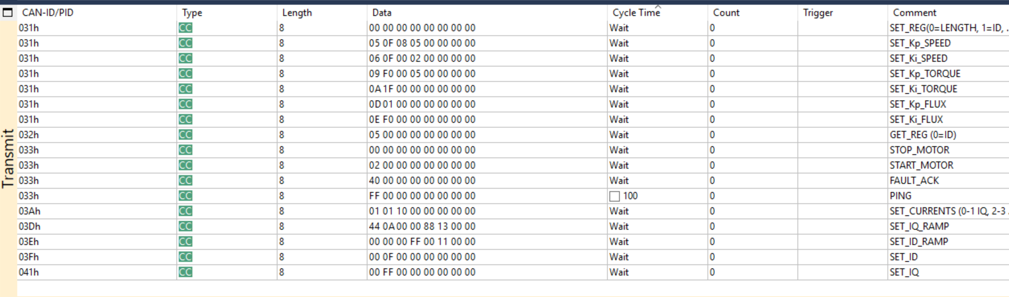
\includegraphics[width=0.88\textwidth]{pcan_rx.png}
\caption{PCAN-View trace of MCU-to-dyno traffic. Identifier \texttt{0x10}
carries ACK/NACK; identifier \texttt{0x11} carries \texttt{REG\_VALUE};
the remaining identifiers are the periodic diagnostic stack.}
\label{fig:pcan-rx}
\end{figure}

The trace in \cref{fig:pcan-rx} confirms three properties at once.

\begin{enumerate}[leftmargin=1.6em]
  \item The physical layer, the bit-rate and the termination are correct:
        frames arrive without error frames and without ACK-slot errors.
  \item \texttt{Send\_Status} is running at the designed period. Counting
        the ten diagnostic identifiers between two occurrences of the
        sequence counter is a direct measurement of the \SI{100}{\milli\second}
        tick.
  \item The ACK/NACK identifier \texttt{0x10} and the \texttt{REG\_VALUE}
        identifier \texttt{0x11} are distinct, which is the observable
        counterpart of \cref{lst:ack}.
\end{enumerate}

A board that fails this test is not ready for command injection. Several
early bring-up failures---wrong bit-rate, missing 120~$\Omega$
termination, TX FIFO left in a non-idle state---were caught here, in
minutes, rather than inside TRACE32.

\section{Command-by-command tracking}
\label{sec:tracking}

For each command the same protocol was followed: inject, halt, step,
resume, compare. The notes below are the ones that changed the code.

\begin{itemize}[leftmargin=1.6em]
  \item \texttt{EXECUTE\_COMMAND 0x33}. The original start/stop complement
        was visible as a \texttt{STOP\_MOTOR} FCP frame being built for a
        CAN payload that had only \texttt{FAULT\_ACK} set. After the
        rewrite of \cref{sec:exec}, a payload with a single flag produces
        a single FCP frame with the matching \texttt{MC\_PROTOCOL\_CMD\_*}
        code.
  \item \texttt{SET\_RAMP 0x37}. Duration and final speed are unpacked
        little-endian; swapping the 16-bit duration bytes is a common
        DBC error and was caught here before the DBC was declared frozen.
  \item \texttt{SET\_CURRENT\_ID / IQ}. The 16-bit signed reconstruction
        was checked with the values \texttt{0x00E8} ($+232$) and
        \texttt{0xFF18} ($-232$) to confirm sign extension.
  \item \texttt{SET\_REG 0x31}. See the next section; this is the case
        that disagreed with the written protocol.
  \item PI round-trip. A \texttt{SET\_REG} of \texttt{SPEED\_KP} with
        numerator $N$ and divisor $n$, followed by a \texttt{GET\_REG} of
        the same register, returned the packed word
        $(n \ll 16) \mid N$ on identifier \texttt{0x11}.
\end{itemize}

\section{Case study: SET\_REG versus the dishwasher specification}
\label{sec:discrepancy}

The Motor Control protocol document~\cite{stmcprotocol} describes
\texttt{SET\_REG} as a length-prefixed frame: byte~0 is the payload
length, byte~1 is the register identifier, the following bytes are the
value. The SR5E1 library, as written and as executed, does something else.
Byte~0 of the CAN payload \emph{is} the register identifier. There is no
length byte on the wire; the FCP length is inserted by DYNO2DW when it
builds \texttt{msg[]}.

\begin{figure}[ht]
\centering
\begin{minipage}[t]{0.48\textwidth}
  \centering
  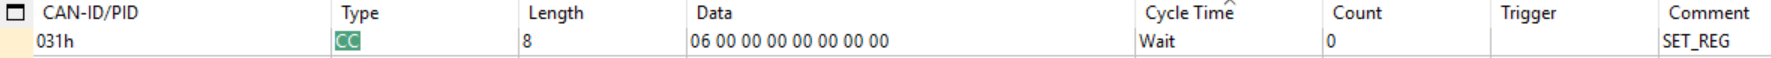
\includegraphics[width=\textwidth]{setreg_pcan.png}
  \captionof{figure}{SET\_REG frame as transmitted from PCAN-View.
  Byte~0 of the payload is already the target register identifier.}
  \label{fig:setreg-pcan}
\end{minipage}\hfill
\begin{minipage}[t]{0.48\textwidth}
  \centering
  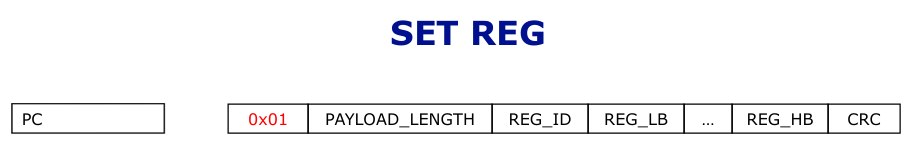
\includegraphics[width=\textwidth]{dw_spec.png}
  \captionof{figure}{SET\_REG layout in the dishwasher protocol
  specification, with a length byte in front of the register identifier.}
  \label{fig:dw-spec}
\end{minipage}
\end{figure}

TRACE32 made the disagreement uncontroversial. Halting in the
\texttt{SET\_REG} case showed \texttt{RxArr[0]} being copied into the
register-id argument of \texttt{UI\_SetReg}, not into \texttt{msg[1]}
as a length. A frame built according to the specification---length first---
wrote the wrong register and returned a NACK or, worse, a silent write
to an unintended PI gain.

Two equally defensible repairs were available: change the firmware to
match the document, or document the firmware and change the DBC. The
second option was taken, for three reasons.

\begin{enumerate}[leftmargin=1.6em]
  \item The library was already deployed on boards that the dyno spoke to.
        Changing the on-wire layout would have broken those boards and
        every recorded trace.
  \item DYNO2DW exists specifically to absorb this kind of difference: the
        FCP frame, with its length byte and CRC, is an internal MCU
        affair. The CAN payload can be denser.
  \item The DBC is the contract the GUI and the dyno software compile. Once
        it says ``byte~0 is \texttt{REGISTER\_ID}'', both consumers are
        right together.
\end{enumerate}

The episode is recorded at this length because it is the standard failure
mode of protocol work: two artefacts that each look consistent, and a bus
that cannot tell them apart until a debugger sits on both sides of the
ISR.

\section{What was considered passing}
\label{sec:pass-criteria}

A command was marked validated when all of the following held on hardware.

\begin{itemize}[leftmargin=1.6em]
  \item The TRACE32 locals showed the intended FCP code, length and
        payload, and a CRC that \texttt{SelfCRCCalc} accepted.
  \item The Motor Control function associated with that code executed
        (verified by a breakpoint on the function itself, not only on
        DYNO2DW).
  \item The bus showed identifier \texttt{0x10} with \texttt{0xF0} for
        writes, or identifier \texttt{0x11} with the expected four-byte
        value for reads.
  \item A second, malformed variant of the same command (truncated DLC,
        reserved flag set, out-of-range register id) produced
        \texttt{0xFF} and did not change machine state.
\end{itemize}

The GUI of \cref{ch:gui} was not used as an oracle during this campaign.
It was connected only after the DBC matched the traces, so that a widget
bug could not be mistaken for a firmware bug.

\chapter{The CAN Database}
\label{ch:dbc}

A DBC file is the human-readable contract of the bus~\cite{vectordbc}.
This chapter describes the DBC that was brought into alignment with the
firmware of \cref{ch:dev}: the message tree, two representative signal
layouts, the offset convention, the reserved window for new commands, and
the structural correction of ACK/NACK.

\section{Role of the DBC in this project}
Without a DBC, CANalyzer displays identifiers and hex dumps. With a DBC it
displays ``heatsink temperature, \SI{47.3}{\celsius}'' and it can encode a
speed ramp from two physical fields, \emph{final speed in RPM} and
\emph{duration in ms}. The Python GUI of \cref{ch:gui} never packs a
CAN frame itself; it writes system variables, CAPL reads those variables,
and CANalyzer encodes the frame from the DBC. It follows that a DBC which
disagrees with the firmware is not a documentation issue. It is a
functional bug in the operator path.

The file therefore defines, for every message,

\begin{itemize}[leftmargin=1.6em]
  \item the 11-bit identifier;
  \item the DLC in bytes;
  \item each signal's start bit, length, signedness, endianness, factor,
        offset and unit;
  \item a comment that names the matching firmware symbol where one
        exists.
\end{itemize}

\section{Message tree}
\label{sec:tree}

The DBC is organised in three branches, visible in CANalyzer's
symbol explorer (\cref{fig:dbc-tree}).

\begin{figure}[ht]
\centering
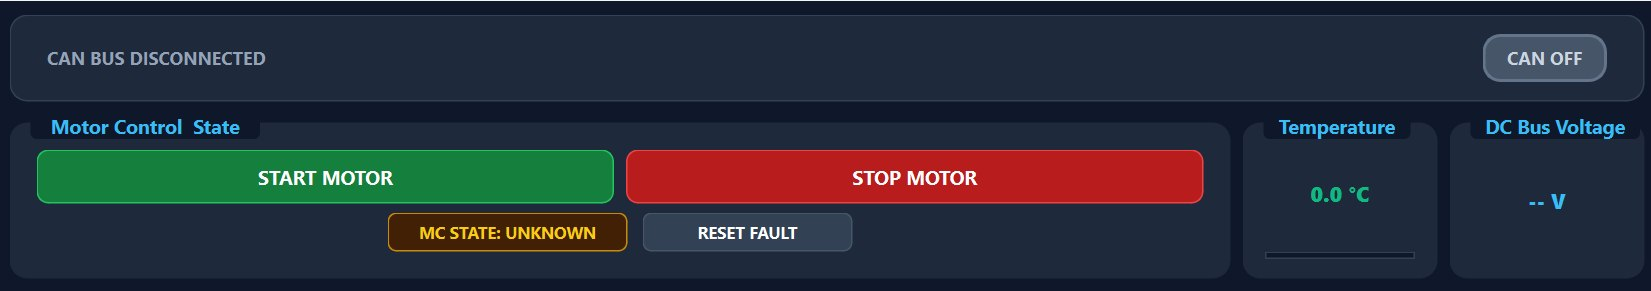
\includegraphics[width=0.72\textwidth]{dbc_tree.png}
\caption{DBC message tree as shown by CANalyzer. Diagnostics occupy
\texttt{0x40}--\texttt{0x60}; motor-control commands occupy
\texttt{0x30}--; MCU responses occupy \texttt{0x10} and \texttt{0x11}.}
\label{fig:dbc-tree}
\end{figure}

\paragraph{Diagnostics, \texttt{0x40}--\texttt{0x60}.}
Ten periodic messages, one per register of \cref{tab:diag-map}. Each has
DLC~4 and a single 32-bit little-endian signal. Factors convert the SDK's
internal units into volts, degrees Celsius, milliamperes or RPM so that
the GUI never sees raw ticks.

\paragraph{Motor-control commands, \texttt{0x30}--.}
\texttt{SET\_REG}, \texttt{GET\_REG}, \texttt{EXECUTE\_COMMAND},
\texttt{SET\_RAMP}, the paired and independent current commands, and the
two current ramps. Layouts are message-specific: a bit-mask, a pair of
physical values, a packed PI word.

\paragraph{MCU responses, \texttt{0x10} and \texttt{0x11}.}
\texttt{ACK\_NACK} and \texttt{REG\_VALUE}. These two messages are the
DBC counterpart of \cref{lst:ack}.

\section{Two representative layouts}
\label{sec:layouts}

\subsection{\texttt{EXECUTE\_COMMAND} (identifier \texttt{0x33})}
The payload is a bit-mask spread over two bytes. Each flag is a 1-bit
signal with factor~1, so CAPL and the GUI can write
\texttt{msg.EXE\_START\_MOTOR = 1} without shifting. The bit positions
match \cref{tab:exec-flags}. Unused bits are present in the DBC as
reserved signals; they are transmitted as zero and ignored on reception,
which is what makes a later extension of the mask binary-compatible.

\subsection{\texttt{SET\_RAMP} (identifier \texttt{0x37})}
Two physical signals share the eight-byte payload:

\begin{itemize}[leftmargin=1.6em]
  \item \texttt{FinalSpeed\_execrmp} --- signed, little-endian, factor
        chosen so that the GUI unit is RPM;
  \item \texttt{Duration\_execrmp} --- unsigned, little-endian, unit
        milliseconds.
\end{itemize}

The same pattern---final value plus duration---is reused for
\texttt{SET\_ID\_RAMP} and \texttt{SET\_IQ\_RAMP}, with the final-value
signal scaled in milliamperes rather than RPM. Reusing the pattern is a
deliberate invitation to reuse CAPL: the speed-ramp event handler of
\cref{lst:capl-speed} has a current-ramp twin that differs only in the
message type.

\begin{figure}[ht]
\centering
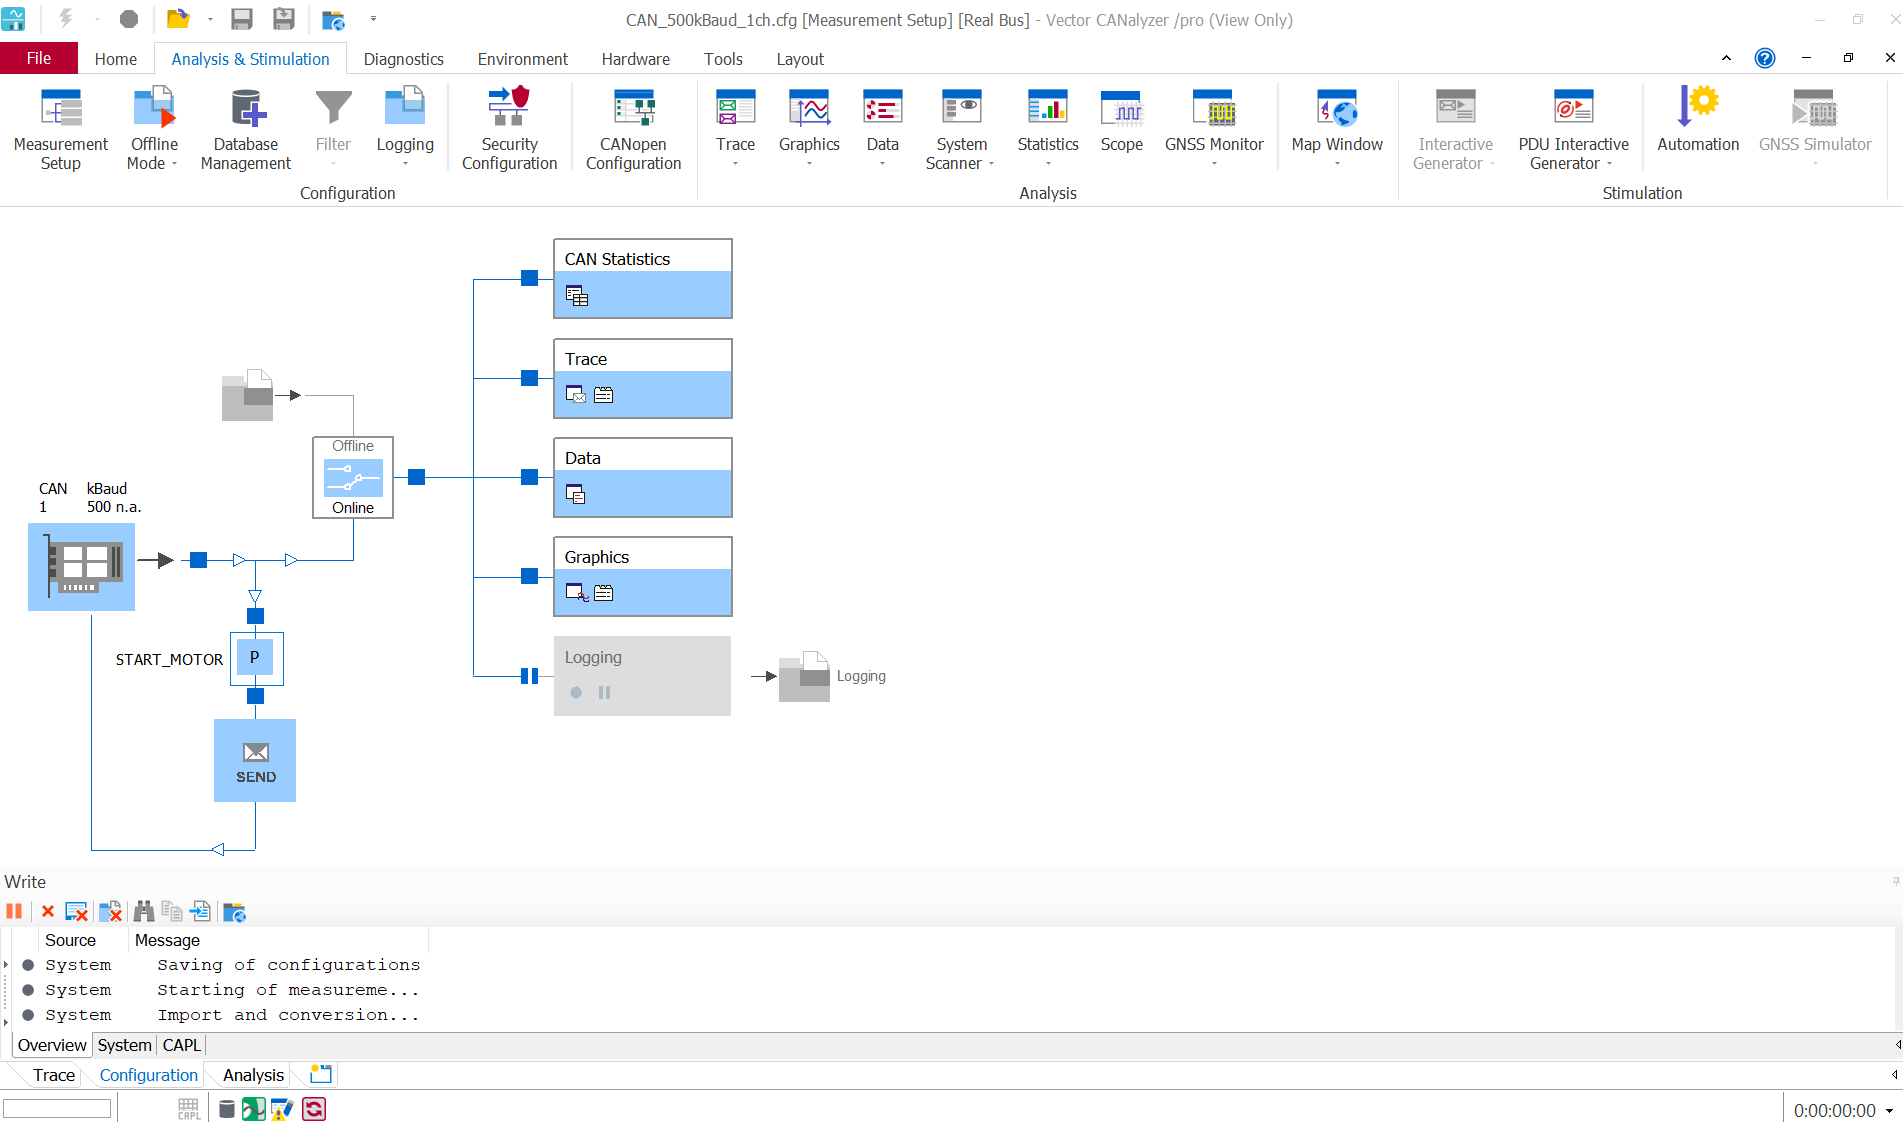
\includegraphics[width=0.95\textwidth]{dbc_signals.png}
\caption{Signal-level view of a DBC message in CANalyzer. Start bit,
length, factor and offset are the fields that must match the firmware's
little-endian packing.}
\label{fig:dbc-signals}
\end{figure}

\section{Alignment with the $+$\texttt{0x30}/$+$\texttt{0x40} rule}
\label{sec:dbc-offset}

The DBC was rewritten so that a reader who knows the firmware offset rule
of \cref{sec:offset} can predict every identifier, and a reader who knows
the DBC can predict every firmware code. Three ranges result.

\begin{center}
\begin{tabular}{lll}
\toprule
Range & Role & Origin \\
\midrule
\texttt{0x10}--\texttt{0x11} & MCU responses & size-based dispatch, \cref{sec:ack} \\
\texttt{0x30}--\texttt{0x3A} & original commands & firmware library as found \\
\texttt{0x3B}--\texttt{0x3C} & \texttt{SET\_CURRENT\_ID} / \texttt{IQ} & added in this work \\
\texttt{0x3E}--\texttt{0x3F} & $I_d$ / $I_q$ ramps & $I_q$ existing, $I_d$ added \\
\texttt{0x40}-- & diagnostics & \texttt{Send\_Status} \\
\bottomrule
\end{tabular}
\end{center}

\texttt{SET\_CURRENT\_ID} and \texttt{SET\_CURRENT\_IQ} illustrate the one
place where the naive offset was not used. The protocol codes
\texttt{0x0F} and \texttt{0x11} would have mapped to \texttt{0x3F} and
\texttt{0x41}. The first collides with \texttt{SET\_IQ\_RAMP}; the second
sits inside the diagnostic window. Unused identifiers \texttt{0x3B} and
\texttt{0x3C} were therefore assigned in both the DBC and the C
\texttt{switch}, and a comment in each artefact points at the other. The
offset rule remains the default; collisions are resolved by an explicit
exception, never by silent reuse.

\section{Structural correction of ACK/NACK}
\label{sec:dbc-ack}

The original DBC declared two messages with identifiers \texttt{0xF0} and
\texttt{0xFF}. Those values are the \emph{payload} of an acknowledgement,
not CAN identifiers: they do not fit in 11 bits without being interpreted
as a different, extended-id convention, and they never appeared on the
wire as identifiers. CANalyzer therefore never decoded a real ACK, and
any CAPL handler attached to those messages was dead code.

\begin{figure}[ht]
\centering
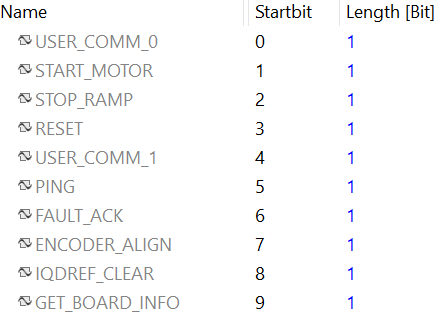
\includegraphics[width=0.55\textwidth]{ack_before.png}
\caption{Original DBC fragment in which \texttt{0xFF} (NACK) and
\texttt{0xF0} (ACK) are declared as distinct CAN identifiers. Both values
are in fact payload codes of the single message \texttt{0x10}.}
\label{fig:ack-before}
\end{figure}

The repair is a single message \texttt{ACK\_NACK} at identifier
\texttt{0x10}, DLC~1, with one unsigned 8-bit signal
\texttt{AckCode}. A value table maps \texttt{0xF0} $\mapsto$
\texttt{ACK} and \texttt{0xFF} $\mapsto$ \texttt{NACK}. Identifier
\texttt{0x11} remains \texttt{REG\_VALUE}, with two 16-bit signals
\texttt{GET\_K\_NUMERATOR} and \texttt{GET\_K\_DENOMINATOR} that mirror
the packing of \cref{sec:pi-pack} for PI reads, and a 32-bit raw signal
for every other register.

After this change, a CAPL \texttt{on message ACK\_NACK} handler fires on
every write, and a CAPL \texttt{on message REG\_VALUE} handler fires on
every read. The Python GUI polls the corresponding system variables and
never has to look at identifiers.

\section{Keeping the DBC honest}
A DBC drifts as soon as a firmware identifier is added without a matching
edit. The working rule adopted at the end of this project is
mechanical and small:

\begin{itemize}[leftmargin=1.6em]
  \item no firmware identifier ships without a DBC message of the same
        name and DLC;
  \item no DBC signal ships without a comment that names the C symbol or
        the bit it corresponds to;
  \item a PCAN-View trace of a newly added message is attached to the
        laboratory notebook before the GUI is allowed to send it.
\end{itemize}

Those three checks would have caught both the ACK-as-identifier mistake
and the SET\_REG length-byte mistake before either reached an operator.

\chapter{CANalyzer Integration and Operator GUI}
\label{ch:gui}

Once the firmware and the DBC agreed, the remaining problem was human.
Composing hexadecimal frames in PCAN-View is the right way to validate a
protocol and the wrong way to run a characterisation campaign. This
chapter describes the operator surface that was built on top of Vector
CANalyzer: a CAPL layer that owns the real-time bus, a COM API that
exports system variables, and a Python GUI that owns widgets, gauges and
plots.

\section{Partition of responsibilities}
\label{sec:partition}

Python is a poor real-time CAN stack. Vector CANalyzer is a poor widget
toolkit. The architecture of \cref{fig:gui-arch} takes that observation
literally.

\begin{figure}[ht]
\centering
\begin{tikzpicture}[
  font=\sffamily\footnotesize,
  box/.style={draw=NavyInk, rounded corners=1.5pt, align=center,
              inner sep=6pt, minimum height=12mm},
  arr/.style={-{Latex}, thick, NavyInk}
]
  \node[box, fill=Paper, minimum width=24mm] (mcu) {Stellar-E\\FDCAN};
  \node[box, fill=Paper, minimum width=28mm, right=12mm of mcu]
    (capl) {CANalyzer\\DBC + CAPL};
  \node[box, fill=Paper, minimum width=28mm, right=12mm of capl]
    (com) {COM API\\sysvars};
  \node[box, fill=Paper, minimum width=24mm, right=12mm of com]
    (py) {Python GUI\\widgets};
  \draw[arr] (mcu) -- node[above, font=\scriptsize] {CAN} (capl);
  \draw[arr] (capl) -- (com);
  \draw[arr] (com) -- (py);
  \draw[arr, dashed] ([yshift=-6mm]py.south) -- ++(0,-5mm) -|
    node[near start, below, font=\scriptsize] {write sysvar}
    ([yshift=-6mm]capl.south);
\end{tikzpicture}
\caption{Operator-path architecture. CANalyzer owns timing, DBC encoding
and CAPL; Python owns the graphical interface and talks only to system
variables via \texttt{win32com.client}.}
\label{fig:gui-arch}
\end{figure}

On startup the Python process instantiates
\texttt{Vector.CANalyzer.Application} through \texttt{win32com.client}
\cite{win32com} and obtains the \texttt{App.SystemVariables} namespace.
From that moment on, two directions of traffic exist.

\paragraph{Bus $\rightarrow$ GUI.}
Firmware emits the ten diagnostic frames and, when asked, a
\texttt{REG\_VALUE}. CAPL \texttt{on message} handlers decode them with
the DBC and write system variables. Python polls those variables on a
timer and refreshes gauges, numeric fields and plots.

\paragraph{GUI $\rightarrow$ bus.}
A button, a slider or a ``Set'' action writes one or more system
variables. A CAPL \texttt{on sysvar} handler wakes, checks the ready
flags described below, fills a typed message and calls
\texttt{output()}. CANalyzer encodes the frame from the DBC and
transmits it.

Python never calls a CAN driver. That single restriction is what makes
the GUI interchangeable: a future operator surface in C\# or in CAPL
panels themselves would reuse the same system variables and the same
DBC.

\begin{figure}[ht]
\centering
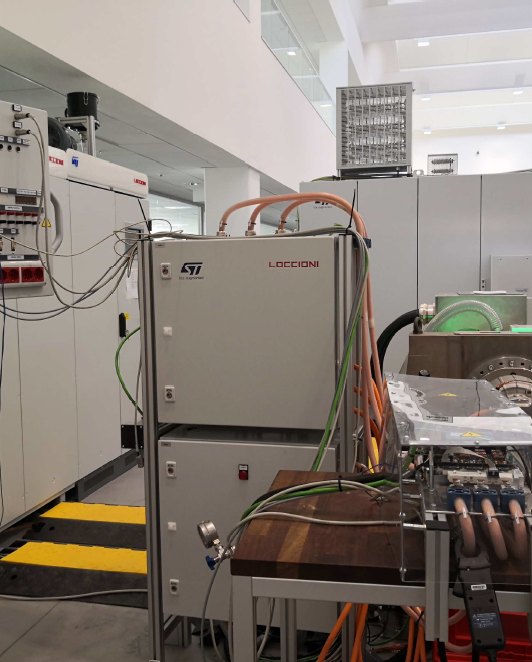
\includegraphics[width=0.95\textwidth]{canalyzer.png}
\caption{Vector CANalyzer during a session, with the system-variable
namespace that the Python GUI reads and writes through the COM API.}
\label{fig:canalyzer}
\end{figure}

\section{Ready flags for multi-parameter commands}
\label{sec:ready}

A speed ramp has two parameters. If the GUI wrote \texttt{SET\_RAMP = 1}
the moment the operator touched either field, the frame on the bus would
carry a stale duration or a stale final speed. The CAPL layer therefore
keeps three variables per multi-parameter command:

\begin{itemize}[leftmargin=1.6em]
  \item a physical value (\texttt{g\_finalSpeed\_value},
        \texttt{g\_durSpeed\_value});
  \item a ready flag per value (\texttt{is\_finalSpeed\_ready},
        \texttt{is\_durSpeed\_ready});
  \item a trigger (\texttt{SET\_SPEED\_RAMP::SET\_RAMP}).
\end{itemize}

The trigger fires the handler; the handler transmits only when every
ready flag is one. The same pattern is used for current ramps and for PI
writes (numerator and divisor). Incomplete edits stay in the GUI and off
the bus.

\begin{lstlisting}[style=caplstyle,caption={CAPL handler for the speed ramp, with ready-flag guard.},label=lst:capl-speed]
on sysvar SET_SPEED_RAMP::SET_RAMP
{
  message SET_RAMP msgSpeedRamp;

  if (@this == 1 &&
      is_finalSpeed_ready == 1 &&
      is_durSpeed_ready   == 1)
  {
    msgSpeedRamp.FinalSpeed_execrmp = g_finalSpeed_value;
    msgSpeedRamp.Duration_execrmp   = g_durSpeed_value;
    output(msgSpeedRamp);
  }
}
\end{lstlisting}

PI writes are factored into a helper, because three loops times two gains
would otherwise copy the same three assignments nine times:

\begin{lstlisting}[style=caplstyle,caption={CAPL helper that encodes a packed PI SET\_REG.},label=lst:capl-pi]
void send_pi_message(word reg_id, int val, int denom)
{
  message SET_REG msg;
  msg.REGISTER_ID           = reg_id;
  msg.REGISTER_VALUE        = val;
  msg.REGISTER_VALUE_DENOM  = denom;
  output(msg);
}
\end{lstlisting}

\section{Telemetry handlers}
\label{sec:tel-capl}

On the inbound side, CAPL is a set of trivial assignments. The DBC has
already unpacked the frame; the handler's only job is to copy the
physical value into a system variable that Python will poll.

\begin{lstlisting}[style=caplstyle,caption={Inbound CAPL: diagnostics and REG\_VALUE.},label=lst:capl-diag]
on message DIAG_TORQUE_REF
{
  @DIAG_MESSAGES::TORQUE_REF = this.DWord(0);
}

on message REG_VALUE
{
  @GET_REG::K_num = this.GET_K_NUMERATOR;
  @GET_REG::K_den = this.GET_K_DENOMINATOR;
}
\end{lstlisting}

Using \texttt{this.DWord(0)} for the raw diagnostic payload is
intentional. Factors and units are applied either in the DBC signal
definition (when the GUI wants physical units) or in Python (when a plot
needs a custom scale). They are never applied in both places.

\section{Operator panels}
\label{sec:panels}

The GUI is organised as a connection banner plus four tabs. The banner is
always visible: a CAN-bus indicator, a machine-state field, heatsink
temperature, DC-link voltage, and the start / stop / reset-fault
controls. Putting those controls outside the tabs is a safety choice. An
operator who is looking at a PI panel can still stop the motor without
changing tab.

\subsection{Motor control panel}
\Cref{fig:gui-overview} is the first surface the operator sees. Start and
stop map onto the \texttt{EXECUTE\_COMMAND} flags of
\cref{tab:exec-flags}. Temperature and DC-link voltage are bound to
\texttt{DIAG\_TEMPERATURE} and \texttt{DIAG\_BUS\_VOLTAGE}. Machine state
is bound to \texttt{DIAG\_STATE\_MC}; the reset-fault button sets
\texttt{FAULT\_ACK}.

\begin{figure}[ht]
\centering
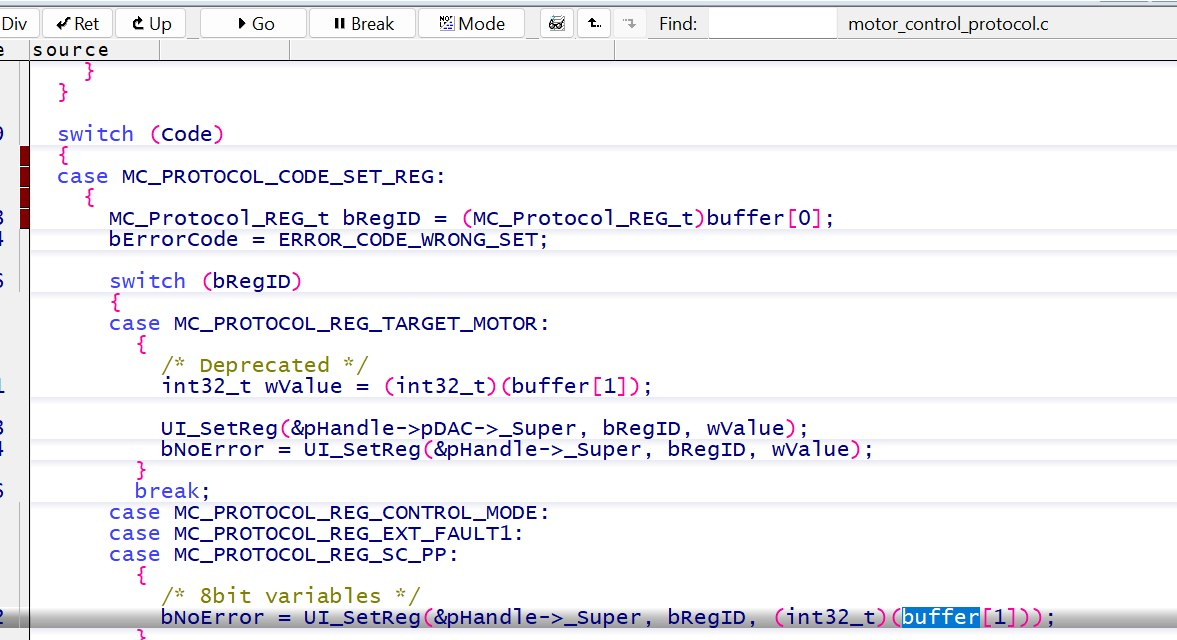
\includegraphics[width=0.95\textwidth]{gui_overview.png}
\caption{Motor control panel. Connection status, start/stop, thermal and
DC-link readouts, machine state and fault reset live in the top banner
so they remain reachable from every tab.}
\label{fig:gui-overview}
\end{figure}

\subsection{Speed control}
The speed tab (\cref{fig:gui-speed}) exposes the two parameters of
\texttt{SET\_RAMP}: final speed in RPM and ramp duration in milliseconds,
plus an apply button that is the trigger of \cref{lst:capl-speed}. A
gauge shows the reference (\texttt{DIAG\_SPEED\_REF}) against the
measured speed (\texttt{DIAG\_SPEED\_MEAS}) so that a ramp in progress is
visible without reading a plot.

\begin{figure}[ht]
\centering
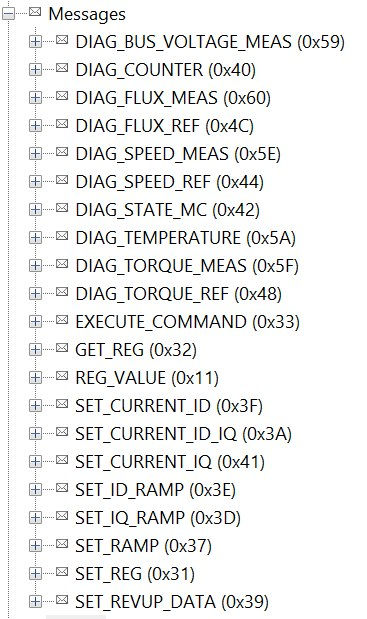
\includegraphics[width=0.95\textwidth]{gui_speed.png}
\caption{Speed-control tab. The operator sets a final speed and a
duration; the gauge compares reference and actual RPM in real time.}
\label{fig:gui-speed}
\end{figure}

\subsection{PI controller}
The PI tab (\cref{fig:gui-pi}) is a direct view of
\cref{sec:pi-pack}. Three groups---speed, flux, torque---each offer $K_p$
and $K_i$ as a numerator and a power-of-two divisor. ``Set'' calls
\texttt{send\_pi\_message} with the corresponding register identifier.
``Read'' issues \texttt{GET\_REG} and fills the same fields from
\texttt{REG\_VALUE}, which is how an operator confirms that a write
round-tripped.

\begin{figure}[ht]
\centering
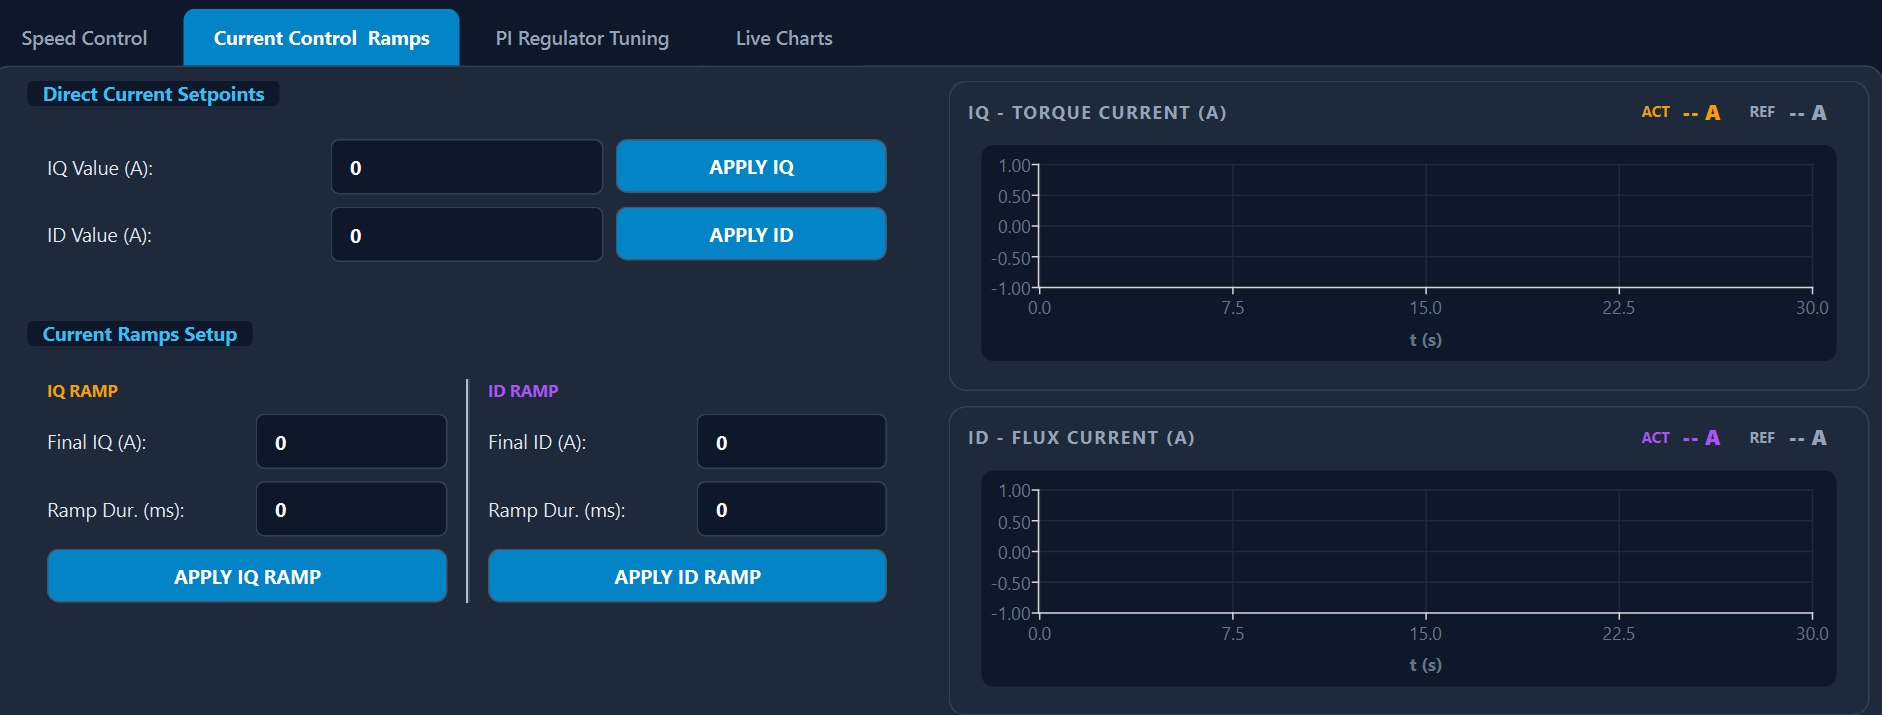
\includegraphics[width=0.95\textwidth]{gui_pi.png}
\caption{PI-controller tab. Each of the three loops exposes $K_p$ and
$K_i$ as a numerator / $2^n$ pair, matching the packed 32-bit register
layout.}
\label{fig:gui-pi}
\end{figure}

\subsection{Current control}
The current tab (\cref{fig:gui-current}) is the operator counterpart of
\cref{sec:id-iq,sec:iq-ramp,sec:id-ramp}. $I_q$ and $I_d$ can be written
as instantaneous set-points or as ramps with their own durations. Two
strip charts show reference against measurement for each axis, which is
the quantity a current-loop tuning session actually looks at.

\begin{figure}[ht]
\centering
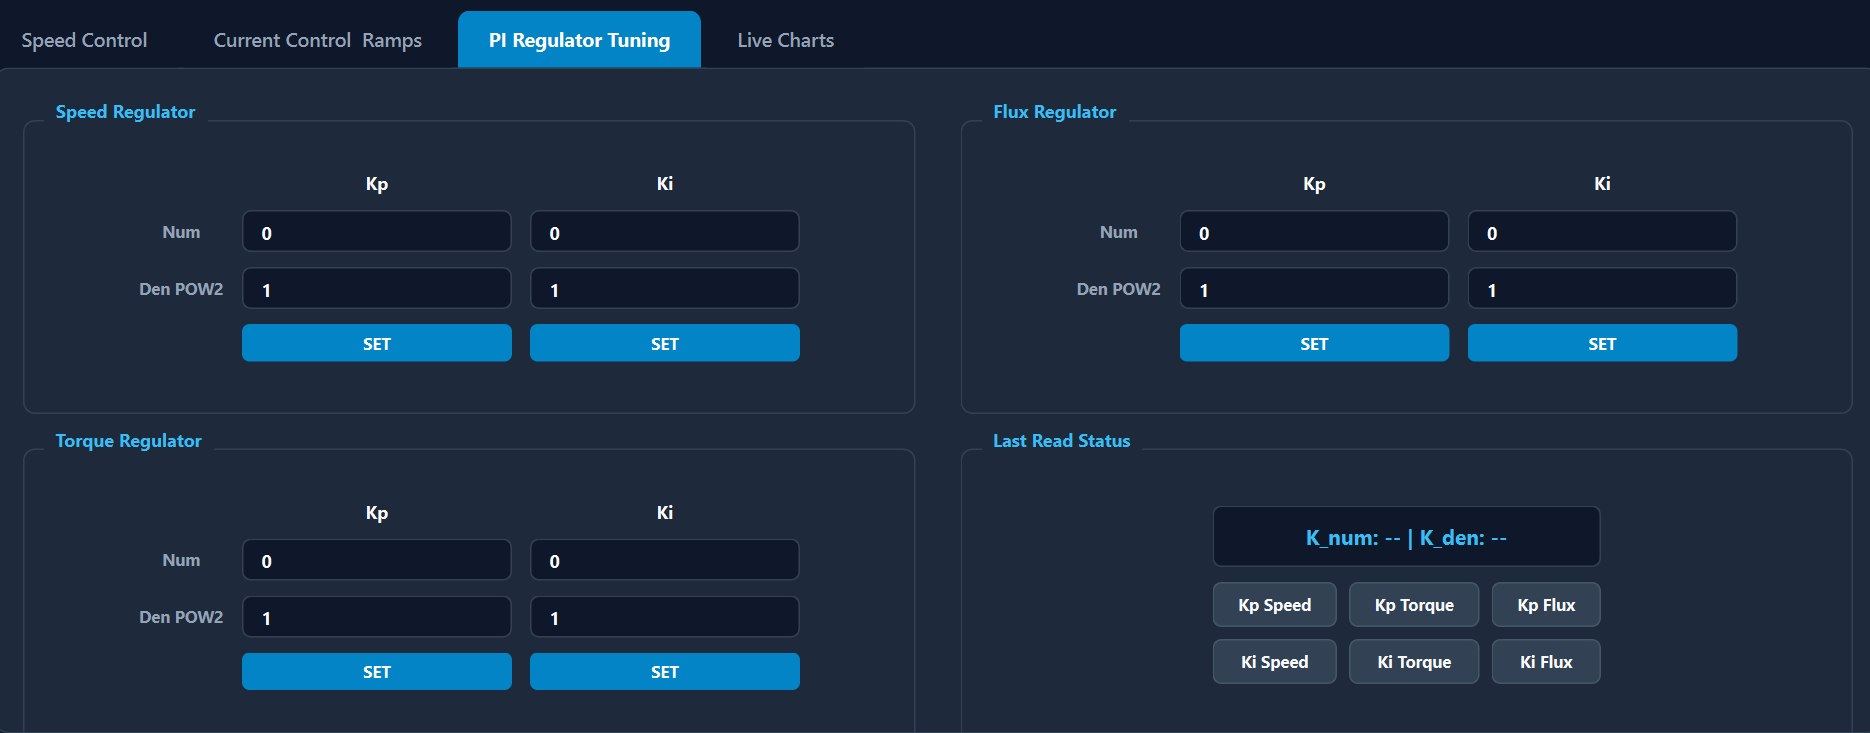
\includegraphics[width=0.95\textwidth]{gui_current.png}
\caption{Current-control tab. Independent $I_q$ and $I_d$ set-points and
ramps, with live plots of reference and measured current on each axis.}
\label{fig:gui-current}
\end{figure}

\subsection{Live charts}
The last tab (\cref{fig:gui-charts}) repeats the speed gauge and the two
current plots at a larger size, without the entry fields. It is the
surface used once a test is running and the operator's job is to watch,
not to command.

\begin{figure}[ht]
\centering
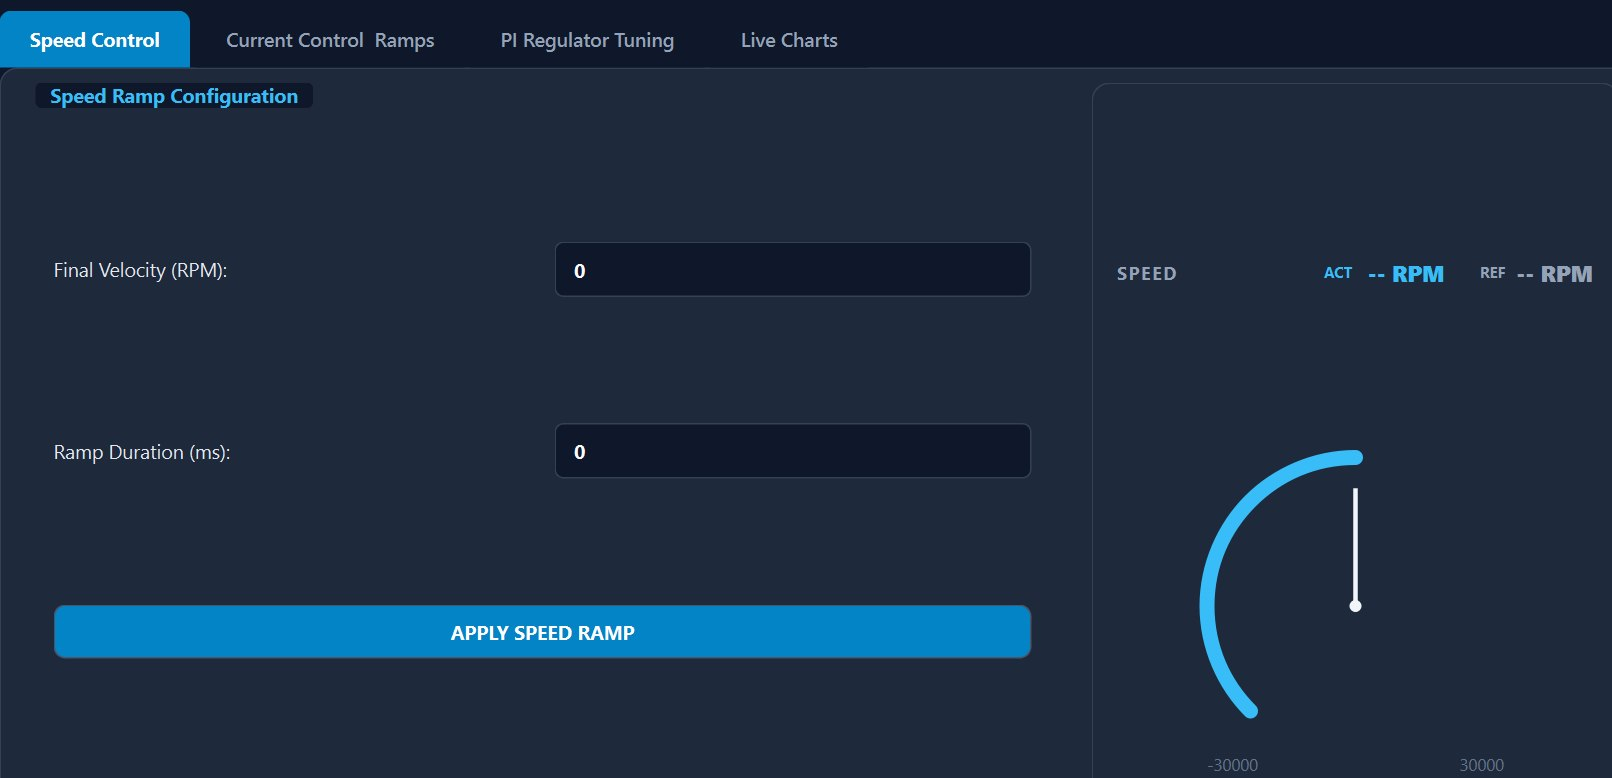
\includegraphics[width=0.95\textwidth]{gui_charts.png}
\caption{Live-charts tab: speed overview together with the $I_q$
(torque) and $I_d$ (flux) current plots.}
\label{fig:gui-charts}
\end{figure}

\section{What the GUI does not do}
A short negative list, because the temptation to grow an operator surface
into a second dyno controller is strong and was resisted.

\begin{itemize}[leftmargin=1.6em]
  \item The GUI does not implement a safety PLC. Emergency stop remains a
        hardware input to the inverter and to the dyno.
  \item The GUI does not log to disk. CANalyzer already records traces in
        a format that the rest of the laboratory toolchain consumes.
  \item The GUI does not re-implement DBC packing. If a signal scale is
        wrong, the fix is in the DBC, not in a Python constant.
  \item The GUI does not talk to the MCU except through CANalyzer. There
        is no second CAN adapter in the Python process, so there is no
        second source of frames to debug.
\end{itemize}

Those restrictions are what keep the three-artefact rule of
\cref{ch:intro} intact: firmware, DBC, operator surface, in that order of
authority.

\chapter{Conclusions and Outlook}
\label{ch:conc}

\section{Results}
The project set out to make the CAN interface between a Stellar-E inverter
and a dynamometer bench automatable. That sentence unpacks into three
artefacts that now agree with each other.

\paragraph{The SR5E1 CAN library is a contract, not a collection of
handlers.}
\texttt{EXECUTE\_COMMAND} commits to a single Motor Control command per
frame. Independent $I_d$ and $I_q$ references exist as first-class codes.
The torque ramp is reachable from CAN, and a flux ramp that the SDK did
not previously offer is implemented through the UI, MCI and STC layers
with the same Q16 increment law as the torque path. PI gains travel as a
packed 32-bit word, numerator and $2^n$ divisor together. ACK/NACK and
\texttt{GET\_REG} no longer share an identifier. Each of those statements
was confirmed on hardware with PCAN-View and TRACE32, not only in
review.

\paragraph{The DBC is a projection of that contract.}
Identifiers follow the $+$\texttt{0x30}/$+$\texttt{0x40} offset rule,
with an explicit exception for the independent current commands where
the naive offset would have collided. Acknowledgement codes
\texttt{0xF0} and \texttt{0xFF} are payload values of message
\texttt{0x10}, not identifiers. Signal layouts---bit-masks, little-endian
physical values, packed PI words---match the C unpacking. The
SET\_REG discrepancy against the dishwasher specification was resolved
by documenting the firmware as authoritative and encoding that layout
in the DBC, rather than by breaking boards already in the field.

\paragraph{An operator can drive the inverter without composing
hexadecimal.}
Vector CANalyzer owns timing and encoding. A Python GUI, talking only
to system variables through the COM API, exposes start/stop, speed
ramps, three PI loops, independent current axes and live plots. CAPL
ready-flags keep incomplete multi-parameter commands off the bus.

Taken together, the chain supports the use-cases that motivated the
work: a speed sweep with a defined duration, a current-loop tuning
session with live $I_d$/$I_q$ charts, a PI write that round-trips, and
a diagnostic stream at \SI{100}{\milli\second} that a CAPL script or
the dyno computer can consume without a human in the loop.

\section{Limitations}
Several limitations are accepted rather than accidental.

\begin{itemize}[leftmargin=1.6em]
  \item The physical layer was validated as CAN~2.0 with 11-bit
        identifiers. The FDCAN peripheral can do more; the DBC and the
        GUI cannot, until someone extends both.
  \item Range checking of current and speed set-points is left to the
        Motor Control SDK. A hostile or mistaken CAPL script can still
        request a value that the regulators will saturate. A future
        saturation layer on the DYNO2DW boundary would make NACKs more
        informative, at the cost of a second source of limits.
  \item The GUI is a Windows process that requires a licensed CANalyzer
        installation. It is the right tool for this laboratory and the
        wrong tool for a headless continuous-integration rack. The
        sysvar/DBC contract, however, is reusable from a CAPL-only
        configuration or from any other COM client.
  \item Functional-safety aspects of Stellar-E (lockstep, watchdog,
        ISO~26262 assumptions) were out of scope. The interface is a
        laboratory automation layer, not a safety element.
\end{itemize}

\section{Outlook}
Three extensions follow naturally from the present contract.

\paragraph{Scripted characterisation.}
With the DBC stable, a CAPL (or Python-COM) script can replay a speed
and current profile, log \texttt{REG\_VALUE} and the diagnostic stack,
and produce a characterisation table without the GUI. The ready-flag
discipline is exactly the guard that such a script needs.

\paragraph{CAN FD and higher-rate telemetry.}
Ten 4-byte messages every \SI{100}{\milli\second} are enough for
operator gauges and tight for a fast current loop. Packing several
registers into a single CAN-FD 64-byte frame, or shortening the period
for a subset of signals, is a DBC-compatible change once the TX path
is measured not to drop stacks under \texttt{FCP\_TRANSFER\_IDLE}
back-pressure.

\paragraph{Bidirectional PI scheduling.}
The packed write of \cref{sec:pi-pack} is atomic per gain. A single
message that writes $K_p$ and $K_i$ of one loop together, or a
read-modify-write of a loop's complete state, would make automated
tuning (relay, Ziegler--Nichols, iterative feedback tuning) less
sensitive to a control period that lands between two CAN frames.

\section{Closing remark}
The technical content of this thesis is a handful of C cases, a DBC
file and a Python window. The engineering content is the refusal to let
those three disagree. A bench that is automated on top of a silently
wrong identifier map is worse than a bench that is operated by hand:
it produces plots that look like measurements and are not. The
debug chain of \cref{ch:val}---inject, halt, step, compare---is the
method that keeps the plots honest, and it is the method this
laboratory can reuse the next time a protocol code is added.


\appendix
\chapter{Extended Listings}
\label{ch:app}

The listings in the main chapters are shortened to the statements that
carry the argument. This appendix reproduces the surrounding functions
at the length that a re-implementer would want.

\section{Periodic diagnostic stack}

\begin{lstlisting}[style=cstyle,caption={Diagnostic register list and Send\_Status sketch.}]
#define CAN_NUM_MSG  10

uint8_t msg_tx_diag_can[CAN_NUM_MSG] = {
    MC_PROTOCOL_REG_UNDEFINED,    /* sequence counter, 100 ms */
    MC_PROTOCOL_REG_SPEED_REF,
    MC_PROTOCOL_REG_TORQUE_REF,
    MC_PROTOCOL_REG_FLUX_REF,
    MC_PROTOCOL_REG_BUS_VOLTAGE,
    MC_PROTOCOL_REG_HEATS_TEMP,
    MC_PROTOCOL_REG_SPEED_MEAS,
    MC_PROTOCOL_REG_TORQUE_MEAS,
    MC_PROTOCOL_REG_FLUX_MEAS,
    MC_PROTOCOL_REG_STATUS
};

uint8_t Send_Status(MCP_Handle_t *pHandle)
{
    if (FCP_TRANSFER_IDLE == pHandle->pFCP->TxFrameState) {
        for (i = 0; i < CAN_NUM_MSG; i++) {
            support_buffer = UI_GetReg(&pHandle->_Super,
                                       msg_tx_diag_can[i], NULL);
            /* pack support_buffer little-endian, ID = reg + 0x40 */
            pHandle->pFCP->TxFrame.Code = code;
            pHandle->pFCP->TxFrame.Size = size;
            DBCCAN_TX_IRQ_Handler(pHandle->pFCP);
        }
    }
    return 0;
}
\end{lstlisting}

\section{Flux-ramp call chain}

\begin{lstlisting}[style=cstyle,caption={Complete UI / MCI / STC flux-ramp chain.}]
__weak bool UI_ExecFluxRamp(UI_Handle_t *pHandle,
                            qd_t Vqd, uint16_t hDurationms)
{
    MCI_Handle_t *pMCI = pHandle->pMCI[pHandle->bSelectedDrive];
    MCI_ExecFluxRamp(pMCI, Vqd, hDurationms);
    return true;
}

__weak void MCI_ExecFluxRamp(MCI_Handle_t *pHandle,
                             qd_t Iqdref, uint16_t hDurationms)
{
    pHandle->lastCommand  = MCI_EXECFLUXTRAMP;
    pHandle->hFinalFlux   = Iqdref.d;
    pHandle->hDurationms  = hDurationms;
    pHandle->CommandState = MCI_COMMAND_NOT_ALREADY_EXECUTED;
}

__weak bool STC_ExecCurrentRamps(SpeednTorqCtrl_Handle_t *pHandle,
                                 int16_t hFinalFlux,
                                 uint16_t hDurationms)
{
    bool     AllowedRange = true;
    uint32_t wAux;
    int32_t  wAux1;
    int16_t  hCurrentReferenceId = STC_GetFluxRef(pHandle);

    if (AllowedRange == true) {
        STC_SetControlMode(pHandle, STC_TORQUE_MODE);
        if (hDurationms == 0u) {
            pHandle->FluxRef             = (int32_t)hFinalFlux * 65536;
            pHandle->RampRemainingStepId = 0u;
            pHandle->IncDecAmountId      = 0;
        } else {
            pHandle->TargetFinalId = hFinalFlux;
            wAux  = (uint32_t)hDurationms
                  * (uint32_t)pHandle->STCFrequencyHz;
            wAux /= 1000u;
            pHandle->RampRemainingStepId = wAux + 1u;
            wAux1  = ((int32_t)hFinalFlux
                    - (int32_t)hCurrentReferenceId) * 65536;
            wAux1 /= (int32_t)pHandle->RampRemainingStepId;
            pHandle->IncDecAmountId = wAux1;
        }
    }
    return AllowedRange;
}
\end{lstlisting}

\section{CAPL command and diagnostic events}

\begin{lstlisting}[style=caplstyle,caption={CAPL command and diagnostic events as deployed.}]
on sysvar SET_SPEED_RAMP::SET_RAMP
{
  message SET_RAMP msgSpeedRamp;
  if (@this == 1 &&
      is_finalSpeed_ready == 1 &&
      is_durSpeed_ready   == 1)
  {
    msgSpeedRamp.FinalSpeed_execrmp = g_finalSpeed_value;
    msgSpeedRamp.Duration_execrmp   = g_durSpeed_value;
    output(msgSpeedRamp);
  }
}

void send_pi_message(word reg_id, int val, int denom)
{
  message SET_REG msg;
  msg.REGISTER_ID          = reg_id;
  msg.REGISTER_VALUE       = val;
  msg.REGISTER_VALUE_DENOM = denom;
  output(msg);
}

on message DIAG_TORQUE_REF
{
  @DIAG_MESSAGES::TORQUE_REF = this.DWord(0);
}

on message REG_VALUE
{
  @GET_REG::K_num = this.GET_K_NUMERATOR;
  @GET_REG::K_den = this.GET_K_DENOMINATOR;
}
\end{lstlisting}


% ---------- bibliography -----------------------------------------------------
\backmatter
\bibliography{thesis}

\end{document}
